\documentclass[11pt,a4paper]{article}

\usepackage[margin=2.3cm]{geometry}
\usepackage[T1]{fontenc}
\usepackage{mathptmx}
\usepackage[scaled=0.92]{helvet}
\usepackage{courier}
\usepackage{microtype}
\usepackage{amsmath,amssymb,amsthm}
\usepackage{booktabs}
\usepackage{tabularx}
\usepackage{xcolor}
\usepackage{tikz}
\usetikzlibrary{arrows.meta,calc,positioning,shapes.geometric,decorations.pathreplacing,patterns,fit}
\usepackage[font=small,labelfont=bf,labelsep=colon]{caption}
\usepackage[font=footnotesize,labelfont=bf]{subcaption}
\usepackage[ruled,vlined,linesnumbered]{algorithm2e}
\usepackage{listings}
\usepackage{enumitem}
\usepackage[hidelinks]{hyperref}
\setcounter{tocdepth}{1}

% ---------------------------------------------------------------- colours and TikZ styles
\definecolor{malec}{HTML}{1F7FD1}
\definecolor{femalec}{HTML}{E0186A}
\definecolor{tracec}{HTML}{2B2F33}
\colorlet{gridc}{black!13}
\colorlet{padfill}{black!6}

\tikzset{
  trace/.style   ={draw=tracec,line width=1.6pt,line cap=round,line join=round},
  thintrace/.style={draw=tracec,line width=1.1pt,line cap=round,line join=round},
  ghost/.style   ={draw=black!35,line width=1.2pt,dashed,line cap=round},
  pad/.style     ={circle,fill=padfill,line width=1.1pt,inner sep=0pt,minimum size=4.4mm,
                   font=\sffamily\bfseries\scriptsize,text=black!85},
  mpad/.style    ={pad,draw=malec},
  fpad/.style    ={pad,draw=femalec},
  npad/.style    ={pad,draw=black!55},
  rootbox/.style ={draw=black!45,rounded corners=1pt,line width=0.6pt,minimum size=5.6mm,inner sep=0pt},
  dot/.style     ={circle,fill=black!70,inner sep=0pt,minimum size=1.6mm},
  box/.style     ={draw=black!60,rounded corners=2pt,align=center,inner sep=4pt,fill=black!6},
  flow/.style    ={-{Stealth[length=2.2mm]},line width=0.7pt,black!70}
}
\newcommand{\gridbg}[4]{\draw[gridc,line width=0.4pt,step={(1,-1)}] (#1,#2) grid (#3,#4);}

% ---------------------------------------------------------------- theorem environments
\newtheorem{definition}{Definition}
\newtheorem{proposition}{Proposition}
\newtheorem{lemma}{Lemma}
\theoremstyle{remark}
\newtheorem{remark}{Remark}

\newcommand{\Z}{\mathbb{Z}}
\newcommand{\pos}{p}
\newcommand{\cheb}[1]{\lVert #1 \rVert_\infty}
\newcommand{\pend}{\operatorname{pend}}
\newcommand{\need}{\operatorname{need}}
\newcommand{\freed}{\varphi}
\newcommand{\landpts}{\Lambda}

\lstset{basicstyle=\ttfamily\small,columns=fullflexible,frame=single,framerule=0.3pt,rulecolor=\color{black!40},
        xleftmargin=4pt,xrightmargin=4pt,aboveskip=6pt,belowskip=6pt}

\SetKwProg{Fn}{Function}{}{}
\SetKw{Break}{break}
\SetKw{KwRet}{return}
\SetKwComment{tcp}{\quad$\triangleright$\ }{}

\begin{document}

\begin{center}
  {\LARGE\bfseries The Electric Board Map Layout Algorithm\par}
  \vspace{4pt}
  {\large Octilinear routing, squeeze compaction and nestled forest packing\par}
  \vspace{18pt}
  {\large Technical description of the implementation in \texttt{electric\_map.html}\\
  (a single-page DHTML application)\par}
\end{center}
\vspace{6pt}

\begin{abstract}
Korst, Pronk and van Wijk's \emph{family metro map} draws family relations in the octilinear style of the London
Underground, with segment orientation encoding gender: orthogonal for women, diagonal for men~\cite{korst2020}. The
\emph{Electric Board Map} carries this style and gender rule over to a printed circuit board: vertices of a forest
become \emph{pads} on grid points, edges become \emph{traces} of unit octilinear steps, and the direction of the last
step into a vertex encodes its gender. The algorithm targets forests made of \emph{large} trees ($\ge 9$ vertices) and
many \emph{small} ones ($\le 3$). Large trees are routed generation by generation with straight, one-bend, dogleg and
chamfered-corner traces, a cost that rewards parallel ``bus'' runs, exact branch-and-bound pruning, and a squeeze pass
that rips up and reroutes the board's sides. Small trees are never routed: they are drawn from straight-only templates
(a two-vertex tree is always one straight trace) and nestled into the gaps of the large trees on a flat board grid.
We define the model, prove its key properties, give all constants, and report measurements.
\end{abstract}

\tableofcontents

%=====================================================================================================================
\section{Introduction}

The family metro map~\cite{korst2020} draws a family as a metro line whose end stations are the parents and whose
intermediate stations are the children; a child that founds a family of its own starts a side line through a
T-junction. All segments are horizontal, vertical or diagonal, consecutive stations on a line are equally spaced, and
the orientation of a station's segment encodes gender: women sit on horizontal or vertical segments, men on
diagonal ones (inspired by the Venus and Mars symbols). The result is a compact, attractive overview that uses
space more efficiently than a layered pedigree chart.

The Electric Board Map keeps three ingredients of that design:
\begin{enumerate}[nosep]
  \item an \textbf{octilinear} drawing style (all segments at multiples of $45^\circ$),
  \item the \textbf{gender rule}, \emph{orthogonal $=$ female, diagonal $=$ male}, and
  \item a \textbf{generation-by-generation} construction from a root,
\end{enumerate}
but replaces the metro-line model by a circuit-board model:
\begin{itemize}[nosep]
  \item the input is any \emph{forest} (several trees, isolated vertices allowed), not only binary family trees;
  \item every edge is drawn individually as a \emph{trace} on an integer grid, so all coordinates are exact;
  \item segments of a trace may have \emph{unequal} lengths: straight, one $45^\circ$ bend, a dogleg, or a
        chamfered $90^\circ$ corner (the way circuit boards turn a corner);
  \item traces may run on \emph{adjacent} grid lines, and the cost rewards such parallel runs (``buses'');
  \item the aim is \emph{compactness} (small board, short traces) rather than equal spacing.
\end{itemize}

\paragraph{Target forests.} The implementation is optimised for one kind of input: forests that consist of
\emph{large} trees ($\ge 9$ vertices) and \emph{small} trees ($\le 3$ vertices, i.e.\ isolated vertices, single
edges and paths of length two); \emph{medium} trees ($4$--$8$ vertices) are rare. Large and medium trees are routed
(Section~\ref{sec:routing}); small trees are drawn from straight-only templates and nestled into or next to the large
trees (Section~\ref{sec:packing}). A tree of two vertices is always drawn as one straight trace without bends.

Figure~\ref{fig:pipeline} shows the overall pipeline; Figure~\ref{fig:example2} shows a typical result.

\begin{figure}[t]
\centering
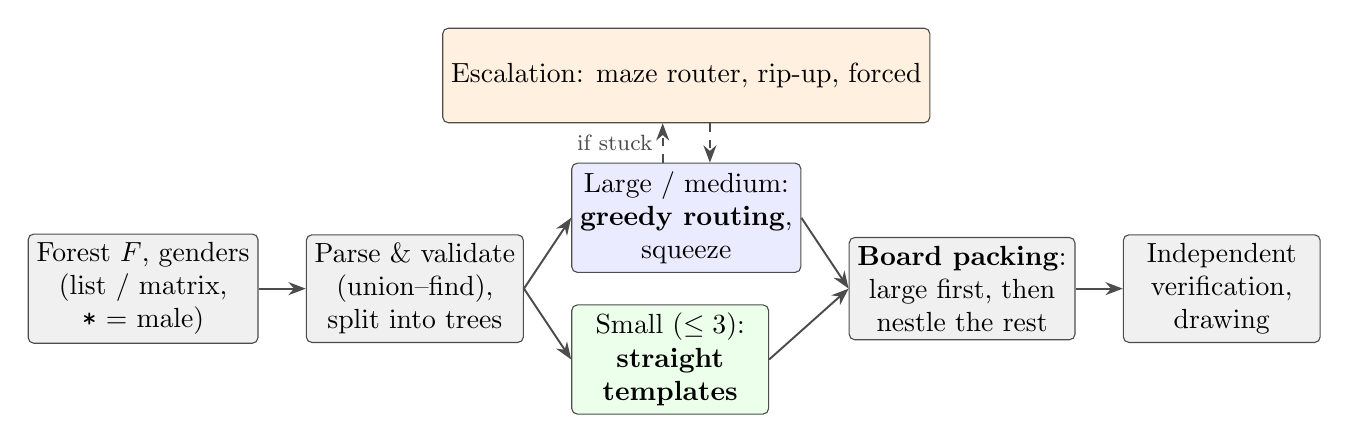
\begin{tikzpicture}[node distance=6mm and 6mm,
    pbox/.style={draw=black!70,rounded corners=2pt,align=center,fill=black!6,minimum width=25mm,minimum height=12mm,inner sep=3pt},
    core/.style={pbox,fill=blue!8},
    opt/.style={pbox,fill=orange!12},
    small/.style={pbox,fill=green!8}]
  \node[pbox] (in)  {Forest $F$, genders\\(list / matrix,\\ \texttt{*} = male)};
  \node[pbox,right=of in] (val) {Parse \& validate\\(union--find),\\split into trees};
  \node[core,right=of val,yshift=9mm] (lay) {Large / medium:\\\textbf{greedy routing},\\squeeze};
  \node[small,right=of val,yshift=-9mm] (tpl) {Small ($\le 3$):\\\textbf{straight}\\\textbf{templates}};
  \node[pbox,right=of lay,yshift=-9mm] (pack){\textbf{Board packing}:\\large first, then\\nestle the rest};
  \node[pbox,right=of pack] (ver){Independent\\verification,\\drawing};
  \node[opt,above=5mm of lay] (fix){Escalation: maze router, rip-up, forced};
  \draw[flow] (in)--(val); \draw[flow] (val.east)--(lay.west); \draw[flow] (val.east)--(tpl.west);
  \draw[flow] (lay.east)--(pack.west); \draw[flow] (tpl.east)--(pack.west); \draw[flow] (pack)--(ver);
  \draw[flow,dashed] ($(lay.north)+(-3mm,0)$) -- node[left,font=\footnotesize]{if stuck} ($(fix.south)+(-3mm,0)$);
  \draw[flow,dashed] ($(fix.south)+(3mm,0)$) -- ($(lay.north)+(3mm,0)$);
\end{tikzpicture}
\caption{Pipeline. Large and medium trees are routed (blue); the escalation steps (orange) are used only when no
simple trace fits. Small trees skip the router (green). Every edit of the graph re-runs the whole pipeline.}
\label{fig:pipeline}
\end{figure}

\paragraph{Outline.}
Section~\ref{sec:model} defines the drawing model and its constraints and proves two basic properties.
Section~\ref{sec:input} covers input and validation. Section~\ref{sec:routing} describes the routing of a large tree:
root and order, candidate traces, legality and reservation, the cost function, escalation, rip-up, multi-start and
the squeeze pass. Section~\ref{sec:packing} describes the small-tree templates and the packing of the forest,
Section~\ref{sec:verify} the verification, Section~\ref{sec:complexity} running time and the exact speed-ups, and
Section~\ref{sec:experiments} measurements. Section~\ref{sec:discussion} discusses limitations.

%=====================================================================================================================
\section{Drawing model}\label{sec:model}

\subsection{Input}
The input is a forest $F=(V,E)$ with $|V|\le 300$ and a gender function $g:V\to\{\mathrm M,\mathrm F\}$.
Each connected component is a tree. For a tree $T$ with a chosen root $r$, every non-root vertex $v$ has a parent
$\operatorname{par}(v)$; $\operatorname{ch}(v)$ is the list of children, $\kappa(v)=|\operatorname{ch}(v)|$, and
$s(v)$ is the number of vertices of the sub-tree rooted at $v$.

\subsection{Grid, directions and traces}
Drawings live on the integer grid $\Z^2$ with the $y$-axis pointing \emph{down} (screen coordinates). The eight
octilinear directions are numbered $k=0,\dots,7$ clockwise on screen:
\[
\begin{aligned}
D_0&=(1,0), & D_1&=(1,1), & D_2&=(0,1), & D_3&=(-1,1),\\
D_4&=(-1,0),& D_5&=(-1,-1),& D_6&=(0,-1),& D_7&=(1,-1).
\end{aligned}
\]
Direction $k$ is \emph{orthogonal} if $k$ is even and \emph{diagonal} if $k$ is odd; turning by one index is a
$45^\circ$ bend. A unit step has length $1$ (orthogonal) or $\sqrt2$ (diagonal); see Figure~\ref{fig:dirs}.

\begin{definition}[Drawing]
A drawing assigns to every vertex $v$ a \emph{pad} $\pos(v)\in\Z^2$ and to every edge $e=\{u,v\}$, with $u$ the
parent of $v$, a \emph{trace} $\pi(e)=(q_0,q_1,\dots,q_n)$ of grid points with $q_0=\pos(u)$, $q_n=\pos(v)$ and
$q_i-q_{i-1}\in\{D_0,\dots,D_7\}$ for all $i$. The points $q_1,\dots,q_{n-1}$ are the \emph{interior points} of the
trace and $q_{n}-q_{n-1}$ is its \emph{arrival direction}.
\end{definition}

\begin{figure}[t]
\centering
\begin{subfigure}[b]{0.36\textwidth}\centering
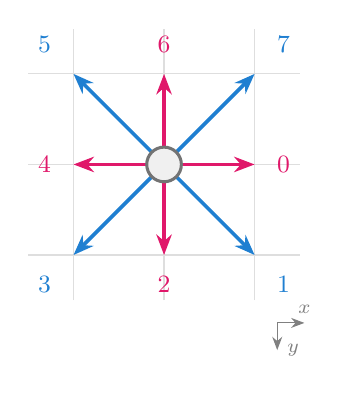
\begin{tikzpicture}[x=1.15cm,y=-1.15cm]
  \gridbg{-1.5}{-1.5}{1.5}{1.5}
  \foreach \k/\dx/\dy in {0/1/0,2/0/1,4/-1/0,6/0/-1}{
     \draw[-{Stealth[length=2.6mm]},line width=1.3pt,femalec] (0,0)--(\dx,\dy);
     \node[font=\small,femalec] at ($1.32*(\dx,\dy)$) {$\k$};}
  \foreach \k/\dx/\dy in {1/1/1,3/-1/1,5/-1/-1,7/1/-1}{
     \draw[-{Stealth[length=2.6mm]},line width=1.3pt,malec] (0,0)--(\dx,\dy);
     \node[font=\small,malec] at ($1.32*(\dx,\dy)$) {$\k$};}
  \node[npad] at (0,0) {};
  \draw[-{Stealth},black!50] (1.25,1.75)--(1.25,2.05) node[right,font=\scriptsize]{$y$};
  \draw[-{Stealth},black!50] (1.25,1.75)--(1.55,1.75) node[above,font=\scriptsize]{$x$};
\end{tikzpicture}
\caption{The 8 directions $D_k$ ($y$ down).}\label{fig:dirs}
\end{subfigure}\hfill
\begin{subfigure}[b]{0.6\textwidth}\centering
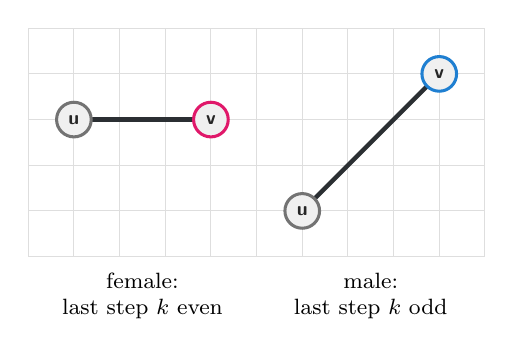
\begin{tikzpicture}[x=0.58cm,y=-0.58cm]
  \gridbg{0}{0}{10}{5}
  \draw[trace] (1,2)--(4,2);  \node[npad] at (1,2) {u}; \node[fpad] at (4,2) {v};
  \draw[trace] (6,4)--(9,1);  \node[npad] at (6,4) {u}; \node[mpad] at (9,1) {v};
  \node[font=\footnotesize,align=center,anchor=north] at (2.5,5.15) {female:\\ last step $k$ even};
  \node[font=\footnotesize,align=center,anchor=north] at (7.5,5.15) {male:\\ last step $k$ odd};
\end{tikzpicture}
\caption{Gender rule on arrival at the child $v$.}\label{fig:gender}
\end{subfigure}
\caption{Directions and the gender rule. Pads are drawn with a magenta ring for female and a blue ring for male
vertices (black: gender irrelevant in the illustration).}
\end{figure}

\subsection{Constraints}
Let $c\in\{2,3\}$ be the \emph{pad clearance}. A drawing is \emph{valid} if
\begin{enumerate}[label=(C\arabic*),leftmargin=3.2em]
  \item\label{c:pad} \textbf{Pad clearance.} $\cheb{\pos(v)-\pos(w)}\ge c$ for all distinct $v,w$ in the same tree
        (pads of different trees are even farther apart, Section~\ref{sec:packing}).
  \item\label{c:excl} \textbf{Exclusive interior points.} An interior point of a trace is neither a pad nor an
        interior point of another trace, and a trace does not visit a grid point twice.
  \item\label{c:diag} \textbf{No crossing diagonals.} No two traces use diagonal steps inside the same unit square.
  \item\label{c:gender} \textbf{Gender rule.} The arrival direction of the trace to $v$ is orthogonal iff
        $g(v)=\mathrm F$ and diagonal iff $g(v)=\mathrm M$.
\end{enumerate}
Traces of different edges may meet only at a common pad (the parent's pad). Note that \ref{c:excl} does \emph{not}
forbid traces on adjacent parallel grid lines: two traces may be one grid step apart, which is what gives the
drawing its board-like density (Figure~\ref{fig:legal}).

\begin{figure}[t]
\centering
\begin{subfigure}[t]{0.24\textwidth}\centering
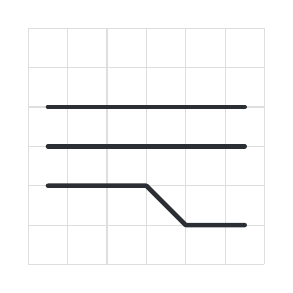
\begin{tikzpicture}[x=0.5cm,y=-0.5cm]
  \gridbg{0}{0}{6}{6}
  \draw[trace] (0.5,2)--(5.5,2); \draw[trace] (0.5,3)--(5.5,3); \draw[trace] (0.5,4)--(3,4)--(4,5)--(5.5,5);
\end{tikzpicture}
\caption{Traces on adjacent grid lines: \emph{allowed}.}
\end{subfigure}\hfill
\begin{subfigure}[t]{0.24\textwidth}\centering
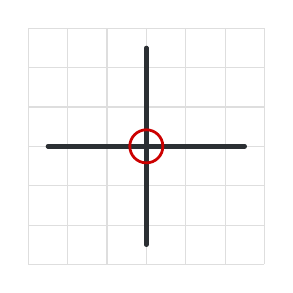
\begin{tikzpicture}[x=0.5cm,y=-0.5cm]
  \gridbg{0}{0}{6}{6}
  \draw[trace] (0.5,3)--(5.5,3); \draw[trace] (3,0.5)--(3,5.5);
  \draw[red!80!black,line width=1pt] (3,3) circle (0.42);
\end{tikzpicture}
\caption{Shared grid point: \emph{forbidden} by \ref{c:excl}.}
\end{subfigure}\hfill
\begin{subfigure}[t]{0.24\textwidth}\centering
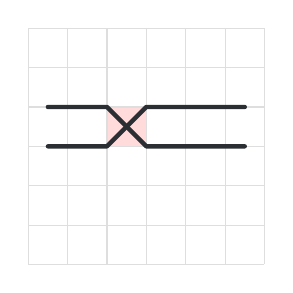
\begin{tikzpicture}[x=0.5cm,y=-0.5cm]
  \fill[red!14] (2,2) rectangle (3,3);
  \gridbg{0}{0}{6}{6}
  \draw[trace] (0.5,2)--(2,2)--(3,3)--(5.5,3);
  \draw[trace] (0.5,3)--(2,3)--(3,2)--(5.5,2);
\end{tikzpicture}
\caption{Diagonals crossing in one unit square: \emph{forbidden} by \ref{c:diag}.}
\end{subfigure}\hfill
\begin{subfigure}[t]{0.24\textwidth}\centering
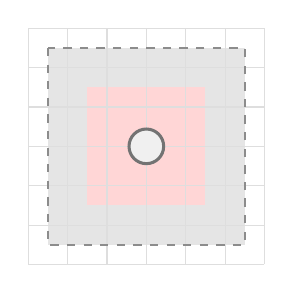
\begin{tikzpicture}[x=0.5cm,y=-0.5cm]
  \fill[black!10] (0.5,0.5) rectangle (5.5,5.5);
  \fill[red!16] (1.5,1.5) rectangle (4.5,4.5);
  \gridbg{0}{0}{6}{6}
  \draw[black!45,dashed,line width=0.6pt] (0.5,0.5) rectangle (5.5,5.5);
  \node[npad] at (3,3) {};
\end{tikzpicture}
\caption{No other pad on the red points ($c{=}2$) or grey points ($c{=}3$).}
\end{subfigure}
\caption{Legality of traces and pads. Because traces may sit on neighbouring grid lines, parallel traces pack
densely; only shared grid points, crossing diagonals and pads closer than the clearance are excluded.}
\label{fig:legal}
\end{figure}

\subsection{Two basic properties}

\begin{proposition}[Planarity]\label{prop:planar}
A drawing satisfying \ref{c:excl} and \ref{c:diag} has no crossings: two traces intersect at most in a common pad.
\end{proposition}
\begin{proof}
Every trace is a union of unit steps between grid points. Two unit steps that share no grid point can intersect
only in the interior of a unit square: orthogonal steps run along grid lines and meet grid lines only at grid
points, while a diagonal step meets the open interior of exactly one unit square and touches its boundary only at its
two end points. Hence an intersection of two steps without a common grid point needs two diagonal steps in the same
unit square, either the two crossing diagonals or the same diagonal twice; both are excluded by~\ref{c:diag}. A
common grid point of two different traces is, by~\ref{c:excl}, never interior to either of them unless it is a pad,
and a pad is shared only by traces incident to that vertex.
\end{proof}

\begin{proposition}[Degree bound]\label{prop:degree}
If $c\ge 2$, a vertex of degree greater than $8$ cannot be drawn validly.
\end{proposition}
\begin{proof}
Consider a pad $\pos(v)$ and an incident trace. Its point next to $\pos(v)$ is at Chebyshev distance $1$; it cannot
be the other end pad because pads are at distance $\ge c\ge2$ \ref{c:pad}, so it is an interior point. By
\ref{c:excl} the interior points of different traces are distinct, so the $\deg(v)$ incident traces use
$\deg(v)$ distinct neighbours of $\pos(v)$, of which there are only eight.
\end{proof}
The implementation draws such vertices anyway and reports the conflicts (Section~\ref{sec:forced}).

%=====================================================================================================================
\section{Input and validation}\label{sec:input}

\paragraph{Adjacency list.} One line per vertex, \texttt{Vertex:Neighbour,Neighbour,...}; an isolated vertex is
written \texttt{D:}. A male vertex is marked with a leading \texttt{*} \emph{wherever} it appears; unmarked vertices
are female. Example (two trees and an isolated vertex):
\begin{lstlisting}
*A:B,*C     B:*A     *C:*A     D:*E,F     *E:D     F:D     G:
\end{lstlisting}
\paragraph{Adjacency matrix.} Row $i$ is vertex $\ell(i)$ with labels $\mathrm{A},\dots,\mathrm{Z},\mathrm{A1},
\dots,\mathrm{Z1},\mathrm{A2},\dots$; a \texttt{*} at the start of a row makes that vertex male.

\paragraph{Validation.} The input is rejected as a whole (and the current graph is kept) if any of the following
occurs; every problem is reported with its line or row:
inconsistent gender marks of the same vertex, malformed lines (not exactly one colon, empty or illegal names, a
\texttt{*} not at the start), a vertex with two lines, a neighbour listed twice, self-loops, asymmetric adjacency
(list or matrix), entries other than $0/1$, a row of wrong length, more than $300$ vertices, and finally cycles. The
forest check uses union--find with path halving over the edge list: an edge whose ends already have the same
representative closes a cycle. The number of successful unions gives the number of trees,
$|V|-\#\text{unions}$. In the visual builder an edge is refused if its ends are already connected (breadth-first
search), so the graph stays a forest at all times.

%=====================================================================================================================
\section{Routing a large tree}\label{sec:routing}

Large and medium trees are routed; this section describes the routing of one such tree.

\subsection{Root and placement order}\label{sec:root}

\paragraph{Root.} If the user names a root in the tree it is used; otherwise the \emph{centre} of the tree is used:
a breadth-first search from the first vertex of the component finds an end $a$ of a longest path, a second search
from $a$ finds the other end $b$, and the middle vertex of the $a$--$b$ path is chosen (the classical tree centre,
cf.\ Jordan~\cite{jordan1869}). (Small trees are not routed, Section~\ref{sec:packing}.) Starting in the centre
minimises the depth of the rooted tree, so the board grows evenly in all directions.

\paragraph{Order.} The tree is rooted by breadth-first search, sub-tree sizes $s(v)$ are computed bottom-up, and the
children of every vertex are sorted by decreasing $s(v)$ (ties by label), so large sub-trees get the best room. The
vertices $u$ are then processed in one of two orders, and for each $u$ all its children are routed one after
another:
\begin{itemize}[nosep]
  \item \textbf{BFS order} (default, ``generation by generation''): like the metro map, one generation is finished
        before the next starts, which yields a radial, balanced board.
  \item \textbf{DFS preorder} (``sub-tree by sub-tree''): a sub-tree is finished before its siblings' sub-trees,
        which clusters families together.
\end{itemize}
The root's pad is placed at $(0,0)$. Throughout the routing the algorithm maintains the occupied pads, the interior
trace points, the used diagonal slots (unit square $\times$ diagonal type), the arrival direction
$\delta_{\mathrm{in}}(v)$ of each placed vertex, the bounding box $B$ of everything drawn, and
$\pend(w)$, the number of children of a placed vertex $w$ that still need a trace.

\begin{algorithm}[t]
\caption{\textsc{LayoutTree}$(T, r, S)$ --- greedy routing of one tree}\label{alg:tree}
\DontPrintSemicolon
root $T$ at $r$ by BFS; compute $s(v)$; sort every $\operatorname{ch}(v)$ by $s$ descending, then label\;
$\mathit{order}\gets$ BFS order of $T$ \textbf{if} $S.\mathit{order}=\text{bfs}$ \textbf{else} DFS preorder\;
$\pos(r)\gets(0,0)$;\quad $\pend(r)\gets\kappa(r)$;\quad $B\gets\{(0,0)\}$\;
\ForEach{$u\in \mathit{order}$}{
  \ForEach{$v\in\operatorname{ch}(u)$}{ \textsc{Route}$(u,v)$ \tcp*{Algorithm~\ref{alg:route}} }
}
\KwRet{pads, traces, $B$, list of forced routes}
\end{algorithm}

\subsection{Candidate traces}\label{sec:candidates}

For the child $v$ of $u$, the first stage enumerates four families of traces starting at $P=\pos(u)$
(Figure~\ref{fig:shapes}); $L$ is the \emph{maximum segment length} (default $6$):
\begin{enumerate}[label=(\alph*),nosep]
  \item \textbf{Straight}: $a$ steps in direction $d_1$, $1\le a\le L$. Arrival direction $d_1$.
  \item \textbf{One bend}: $a$ steps in $d_1$, then $b$ steps in $d_2=d_1+s$, $s=\pm1$, $1\le a,b\le L$.
        Arrival direction $d_2$.
  \item \textbf{Dogleg (jog)}: $a$ steps in $d_1$, $c'$ steps in $d_2=d_1+s$ with $1\le c'\le 3$, and $b$ steps
        in $d_1$ again, $1\le a,b\le L$. Arrival direction $d_1$. This is the PCB offset: a short sideways shift
        between two parallel runs.
  \item \textbf{Chamfered corner}: $a$ steps in $d_1$, $c'$ steps in $d_2=d_1+s$ with $1\le c'\le 3$, and $b$ steps
        in $d_3=d_1+2s$. The trace turns by $90^\circ$ in two $45^\circ$ bends, the way real boards turn a corner
        (no sharp $90^\circ$ corners). Arrival direction $d_3$.
\end{enumerate}
All segment lengths are chosen independently, unlike the equal spacing of the metro map. The gender rule
\ref{c:gender} is applied as a filter on the arrival direction: a female child needs an even arrival direction, a
male child an odd one. Since $d_1\pm1$ has the opposite parity of $d_1$, a single bend always switches between
orthogonal and diagonal, so for every child both the families (a), (c), (d) (last segment with the parity of $d_1$)
and family (b) remain available. Only $45^\circ$ bends are generated in this stage; a $90^\circ$ turn without
chamfer appears only in the maze router, at a high cost (Section~\ref{sec:maze}). Families (c) and (d) can be switched
off together (``two-bend traces'').

\begin{figure}[t]
\centering
\begin{subfigure}[b]{0.19\textwidth}\centering
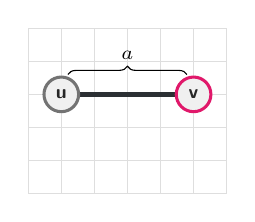
\begin{tikzpicture}[x=0.42cm,y=-0.42cm]
  \gridbg{0}{0}{6}{5}
  \draw[trace] (1,2)--(5,2); \node[npad] at (1,2){u}; \node[fpad] at (5,2){v};
  \draw[decorate,decoration={brace,amplitude=3pt}] (1.2,1.4)--(4.8,1.4) node[midway,above=2pt,font=\scriptsize]{$a$};
\end{tikzpicture}
\caption{Straight, female.}
\end{subfigure}\hfill
\begin{subfigure}[b]{0.19\textwidth}\centering
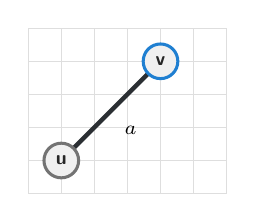
\begin{tikzpicture}[x=0.42cm,y=-0.42cm]
  \gridbg{0}{0}{6}{5}
  \draw[trace] (1,4)--(4,1); \node[npad] at (1,4){u}; \node[mpad] at (4,1){v};
  \node[font=\scriptsize] at (3.1,3.1){$a$};
\end{tikzpicture}
\caption{Straight, male.}
\end{subfigure}\hfill
\begin{subfigure}[b]{0.19\textwidth}\centering
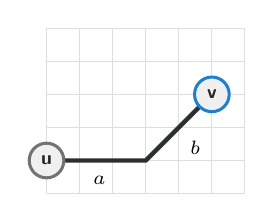
\begin{tikzpicture}[x=0.42cm,y=-0.42cm]
  \gridbg{0}{0}{6}{5}
  \draw[trace] (0,4)--(3,4)--(5,2); \node[npad] at (0,4){u}; \node[mpad] at (5,2){v};
  \node[font=\scriptsize] at (1.6,4.6){$a$}; \node[font=\scriptsize] at (4.5,3.6){$b$};
\end{tikzpicture}
\caption{One bend, male.}
\end{subfigure}\hfill
\begin{subfigure}[b]{0.19\textwidth}\centering
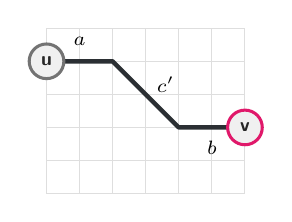
\begin{tikzpicture}[x=0.42cm,y=-0.42cm]
  \gridbg{0}{0}{6}{5}
  \draw[trace] (0,1)--(2,1)--(4,3)--(6,3); \node[npad] at (0,1){u}; \node[fpad] at (6,3){v};
  \node[font=\scriptsize] at (1,0.4){$a$}; \node[font=\scriptsize] at (3.6,1.7){$c'$}; \node[font=\scriptsize] at (5,3.6){$b$};
\end{tikzpicture}
\caption{Dogleg, female.}
\end{subfigure}\hfill
\begin{subfigure}[b]{0.19\textwidth}\centering
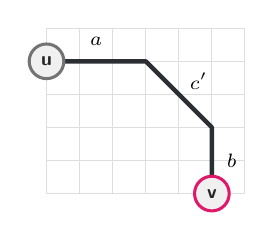
\begin{tikzpicture}[x=0.42cm,y=-0.42cm]
  \gridbg{0}{0}{6}{5}
  \draw[trace] (0,1)--(3,1)--(5,3)--(5,5); \node[npad] at (0,1){u}; \node[fpad] at (5,5){v};
  \node[font=\scriptsize] at (1.5,0.4){$a$}; \node[font=\scriptsize] at (4.6,1.6){$c'$}; \node[font=\scriptsize] at (5.6,4){$b$};
\end{tikzpicture}
\caption{Chamfered corner.}
\end{subfigure}
\caption{The candidate families. Segment lengths are independent; the parity of the last segment decides which
gender the trace can serve.}
\label{fig:shapes}
\end{figure}

\paragraph{Incremental enumeration.} The candidates are generated by a depth-first walk that extends the current
path one unit step at a time (\texttt{walk}/\texttt{stepTo}) and undoes the step afterwards (\texttt{unstep}).
A step that is illegal (Section~\ref{sec:legal}) ends the current segment, so all longer candidates sharing that
prefix are pruned immediately. Each complete candidate is passed to the evaluation (Section~\ref{sec:cost}); a
branch-and-bound test (Section~\ref{sec:complexity}) stops a walk as soon as no extension can beat the best
candidate found so far.

\subsection{Legality and the reservation rule}\label{sec:legal}

A unit step to a point $q$ in direction $k$ is \emph{free} if $q$ is not a pad, not an interior trace point, not
already on the current candidate, and---if $k$ is odd---neither diagonal slot of the unit square crossed by the step
is in use. A candidate ending in $e$ is accepted for evaluation if, in addition, $e$ is not an interior trace point
and no pad lies within Chebyshev distance $c-1$ of $e$ (this includes $\pos(u)$, so the child is at least $c$ away
from its parent). These rules enforce \ref{c:pad}--\ref{c:gender} for every committed trace.

\paragraph{Free directions and landing points.} For a placed pad $w$ let
\begin{align*}
\freed(w) &= \#\{k : \pos(w)+D_k \text{ is free and, for odd } k, \text{ the crossing diagonal slot is unused}\},\\
\landpts(w) &= \#\{q : \cheb{q-\pos(w)}=2,\ q \text{ free},\ \text{no pad other than } w \text{ within distance } c-1 \text{ of } q\}.
\end{align*}
$\freed(w)$ counts the exits still available at $w$ (Proposition~\ref{prop:degree} shows each child needs one);
$\landpts(w)$ counts nearby points where a child pad of $w$ could still land.

\paragraph{Reservation.} Greedy routing has a typical failure: a trace for one vertex wanders past another pad $w$
and takes the last exits that $w$ needs for its own, not yet routed children. To prevent this, define
$\need(w)=\pend(w)$ for $w\ne u$ and $\need(u)=\pend(u)-1$ (the trace being routed is one of $u$'s pending
children). While a candidate is extended, every new point $q$ is charged to the waiting pads around it
(Figure~\ref{fig:reserve}):
\begin{itemize}[nosep]
  \item a pad $w$ with $\cheb{q-\pos(w)}=1$ and $\need(w)>0$ receives one \emph{hit}; the step is refused if
        $\freed(w)-\mathrm{hits}(w)<\need(w)$ afterwards;
  \item a pad $w\neq u$ with $\cheb{q-\pos(w)}=2$ and $\need(w)>0$ receives one \emph{landing hit}; the step is refused
        if $\landpts(w)-\mathrm{landHits}(w)<\need(w)$ afterwards.
\end{itemize}
$\freed$ and $\landpts$ are evaluated once per child on the committed state (cached), and hits are counted per
candidate and undone with the step. The rule is conservative (a point may be counted for several pads), but it is
cheap and removes most dead ends of the greedy order. The ring test is skipped for $u$ itself because the new child
pad usually lands at distance $2$ from its parent.

\begin{figure}[t]
\centering
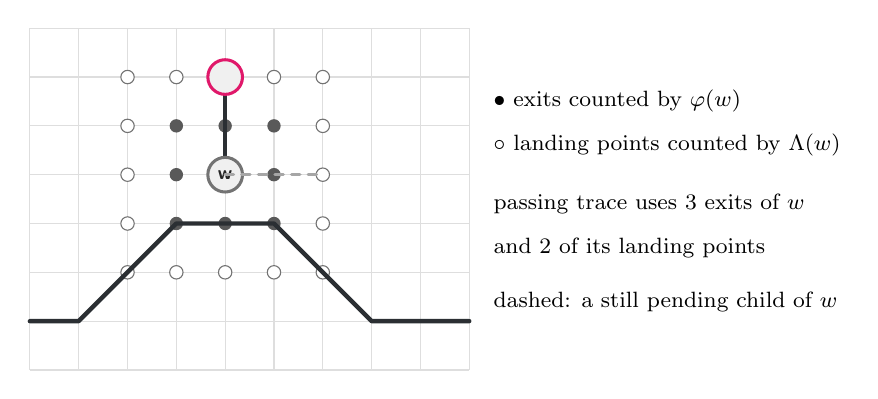
\begin{tikzpicture}[x=0.62cm,y=-0.62cm]
  \gridbg{0}{0}{9}{7}
  % landing ring
  \foreach \dx in {-2,...,2}{\foreach \dy in {-2,...,2}{
     \pgfmathtruncatemacro{\m}{max(abs(\dx),abs(\dy))}
     \ifnum\m=2 \node[circle,draw=black!55,fill=white,inner sep=0pt,minimum size=1.7mm] at (4+\dx,3+\dy){};\fi
     \ifnum\m=1 \node[circle,fill=black!65,inner sep=0pt,minimum size=1.7mm] at (4+\dx,3+\dy){};\fi }}
  % existing trace of another edge passing by
  \draw[trace] (0,6)--(1,6)--(3,4)--(5,4)--(7,6)--(9,6);
  \draw[trace] (4,3)--(4,1);   % the already routed child of w
  \node[npad] at (4,3) {w};
  \node[fpad] at (4,1) {};
  \draw[ghost] (4,3)--(6,3);
  \node[font=\footnotesize,align=left,anchor=west] at (9.3,1.5) {$\bullet$ exits counted by $\freed(w)$};
  \node[font=\footnotesize,align=left,anchor=west] at (9.3,2.4) {$\circ$ landing points counted by $\landpts(w)$};
  \node[font=\footnotesize,align=left,anchor=west] at (9.3,3.6) {passing trace uses 3 exits of $w$};
  \node[font=\footnotesize,align=left,anchor=west] at (9.3,4.5) {and 2 of its landing points};
  \node[font=\footnotesize,align=left,anchor=west] at (9.3,5.6) {dashed: a still pending child of $w$};
\end{tikzpicture}
\caption{Reservation around a pad $w$ with pending children. A candidate trace passing near $w$ is accepted only
if the remaining exits $\freed(w)$ and landing points $\landpts(w)$ stay at least $\need(w)$.}
\label{fig:reserve}
\end{figure}

\subsection{Cost function}\label{sec:cost}

Every legal candidate $\pi$ for the child $v$ of $u$, ending in $e$, with first direction $d_1$ and $b(\pi)$ bends,
receives the cost
\begin{equation}\label{eq:cost}
\begin{split}
C(\pi)\;=\;& \ell(\pi) \;-\; \sigma\,\mathrm{bus}(\pi) \;+\; 0.7\,b(\pi) \;+\; \lambda\,\Delta H(\pi)
  \;+\; 60\,\bigl[\kappa(v)-\freed'(e)\bigr]^+ \;+\; \mu\,\bigl[W(v)-\rho(e)\bigr]^+\\
 &-\; \mathbf 1\bigl[d_1=\delta_{\mathrm{in}}(u)\bigr] \;-\; \omega\bigl(\cheb{e}-\cheb{\pos(u)}\bigr)
  \;+\; 400\,\chi(\pi),
\end{split}
\end{equation}
where $[x]^+=\max(0,x)$ and the cheapest candidate wins (ties go to the first one enumerated). The terms are:
\begin{description}[leftmargin=1.2em,font=\normalfont\itshape]
\item[Length] $\ell(\pi)$: number of orthogonal steps plus $\sqrt2$ times the number of diagonal steps.
\item[Bus bonus] $\mathrm{bus}(\pi)$ is the number of steps of $\pi$ that run parallel to an already committed trace
  on a neighbouring grid line (Figure~\ref{fig:bus}); the weight $\sigma$ is the user's \emph{bus bundling}
  (default $0.5$). For every grid point the implementation keeps, per orientation $o=k\bmod 4$ (``$-$'', ``$\backslash$'',
  ``$|$'', ``$/$''), the number of committed steps of that orientation touching the point. A step $q\to q'$ of
  orientation $o$ counts if, for one of the two neighbouring parallel lines (offset $(0,\pm1)$ for $o=0$, offset
  $(\pm1,0)$ otherwise), both $q$ and $q'$ shifted onto that line touch a committed step of orientation $o$. Traces
  are thereby pulled into dense parallel bundles that turn together, like the buses of a circuit board.
\item[Bends] $0.7$ per $45^\circ$ bend; a two-bend trace costs $1.4$, so it is chosen only when it pays off.
\item[Compactness] $\Delta H$ is the growth of the half perimeter $(x_{\max}-x_{\min})+(y_{\max}-y_{\min})$ of the
  bounding box $B$ if the candidate is added; the corner points of the trace suffice to compute it. The weight
  $\lambda$ is the user's \emph{compactness} (default $1.5$).
\item[Exit look-ahead] $\freed'(e)$ is the number of free directions at the new pad, counting points of the
  candidate itself as blocked. If $v$ has more children than exits, each missing exit costs $60$.
\item[Room look-ahead] Only for $s(v)>1$. With radius $R(v)=\min\bigl(R_{\max},\max(2,\lceil0.9\sqrt{s(v)}\,\rceil)\bigr)$,
  $\rho(e)$ counts free grid points in the $(2R+1)\times(2R+1)$ window around $e$, and the wanted room is
  $W(v)=\min\bigl(\beta\,(s(v)-1),\;0.85\,((2R+1)^2-1)\bigr)$. Defaults: $\beta=1.5$ free points per descendant,
  $\mu=1$, $R_{\max}=2$. This steers big sub-trees towards open space.
\item[Line continuation] A bonus of $1$ if the trace leaves $u$ in the direction in which $u$ itself was reached,
  as in the metro map, where a line runs straight through a station.
\item[Radial growth] A reward of $\omega$ per step of Chebyshev distance gained away from the root (at $(0,0)$).
  It is $0$ by default and $0.6$ in the ``radial'' variant of the multi-start (Section~\ref{sec:multistart}).
\item[Collisions] $\chi(\pi)$ is the number of conflicts the candidate accepts; it is non-zero only in the forced
  mode of Section~\ref{sec:forced}.
\end{description}

\begin{figure}[t]
\centering
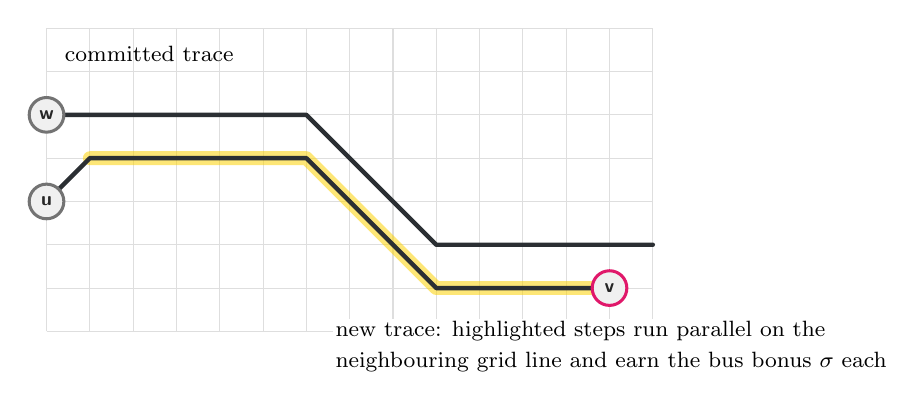
\begin{tikzpicture}[x=0.55cm,y=-0.55cm]
  \gridbg{0}{0}{14}{7}
  \draw[trace] (0,2)--(6,2)--(9,5)--(14,5);
  \node[npad] at (0,2){w};
  \draw[line width=5pt,yellow!70!orange,opacity=0.55,line cap=round,line join=round] (1,3)--(6,3)--(9,6)--(13,6);
  \draw[trace] (0,4)--(1,3)--(6,3)--(9,6)--(13,6);
  \node[npad] at (0,4){u}; \node[fpad] at (13,6){v};
  \node[font=\footnotesize,anchor=west,align=left] at (0.2,0.6) {committed trace};
  \node[font=\footnotesize,anchor=west,align=left,fill=white,inner sep=1pt] at (6.6,7.0) {new trace: highlighted steps run parallel on the};
  \node[font=\footnotesize,anchor=west,align=left,fill=white,inner sep=1pt] at (6.6,7.7) {neighbouring grid line and earn the bus bonus $\sigma$ each};
\end{tikzpicture}
\caption{Bus bonus. The trace from $u$ to $v$ follows the committed trace one grid line below it, including the
diagonal run, so the two turn together; every highlighted step lowers its cost by $\sigma$.}
\label{fig:bus}
\end{figure}

\subsection{Escalation: longer segments and the maze router}\label{sec:maze}

The procedure \textsc{FindRoute} (Algorithm~\ref{alg:find}) escalates when no candidate is legal:
first the enumeration with $L$ and two-bend traces (if enabled), then with $2L$ without them, then a maze router.

\paragraph{Maze router.} The maze router is a Lee/Dijkstra search~\cite{lee1961,dijkstra1959} on states
$(q,k)$ = (grid point, direction of arrival at $q$), so that the cost of a turn is known. From $(q,k)$ the next
direction may be $k$ (cost $0$), $k\pm1$ ($45^\circ$, cost $0.7$) or $k\pm2$ ($90^\circ$, cost $3.0$, deliberately
expensive because a board chamfers its corners); sharper turns are not allowed (Figure~\ref{fig:maze}). A move costs
its step length plus the turn cost plus a soft reservation cost of $2$ for every waiting pad at distance $1$ and $1$
for every waiting pad $w\ne u$ at distance $2$, minus the bus bonus of the step (capped so that every move still costs
at least $0.2$, which keeps Dijkstra's algorithm correct); the hard reservation test of Section~\ref{sec:legal}
applies with a single hit. The goal test accepts the first popped state whose arrival direction has the right parity
and whose point respects the clearance; in the \emph{strict} run it must also offer at least $\kappa(v)$ free
directions. A strict run is tried first, then a non-strict one, each limited to $60\,000$ expansions.

\begin{figure}[t]
\centering
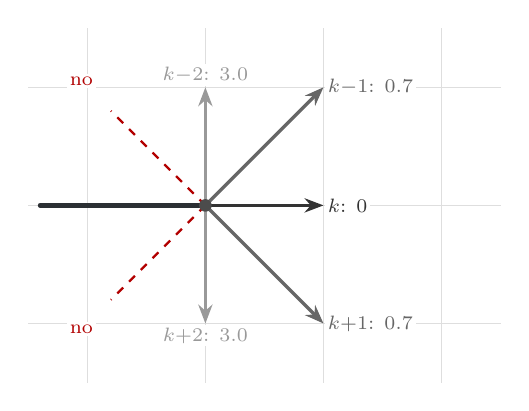
\begin{tikzpicture}[x=1.5cm,y=-1.5cm]
  \gridbg{-1.5}{-1.5}{2.5}{1.5}
  \draw[trace] (-1.4,0)--(0,0);
  \draw[-{Stealth[length=2.4mm]},line width=1.2pt,black!80] (0,0)--(1,0) node[right,font=\scriptsize,fill=white,inner sep=1pt]{$k$: $0$};
  \draw[-{Stealth[length=2.4mm]},line width=1.2pt,black!60] (0,0)--(1,1) node[right,font=\scriptsize,fill=white,inner sep=1pt]{$k{+}1$: $0.7$};
  \draw[-{Stealth[length=2.4mm]},line width=1.2pt,black!60] (0,0)--(1,-1) node[right,font=\scriptsize,fill=white,inner sep=1pt]{$k{-}1$: $0.7$};
  \draw[-{Stealth[length=2.4mm]},line width=1.2pt,black!40] (0,0)--(0,1) node[below,font=\scriptsize,fill=white,inner sep=1pt]{$k{+}2$: $3.0$};
  \draw[-{Stealth[length=2.4mm]},line width=1.2pt,black!40] (0,0)--(0,-1) node[above,font=\scriptsize,fill=white,inner sep=1pt]{$k{-}2$: $3.0$};
  \draw[red!70!black,line width=0.8pt,dashed] (0,0)--(-0.8,0.8); \draw[red!70!black,line width=0.8pt,dashed] (0,0)--(-0.8,-0.8);
  \node[font=\scriptsize,red!70!black,fill=white,inner sep=1pt] at (-1.05,1.05){no}; \node[font=\scriptsize,red!70!black,fill=white,inner sep=1pt] at (-1.05,-1.05){no};
  \node[dot] at (0,0){};
\end{tikzpicture}
\caption{Moves of the maze router from a state reached in direction $k$ (here $k=0$) with their turn penalties
(added to the step length). Turns of $135^\circ$ and $180^\circ$ are not allowed; unchamfered $90^\circ$ turns are
expensive.}
\label{fig:maze}
\end{figure}

\begin{algorithm}[t]
\caption{\textsc{FindRoute}$(u,v,\mathit{allowConflicts})$}\label{alg:find}
\DontPrintSemicolon
\ForEach{$L'\in(L,\,2L)$}{
  enumerate straight, one-bend and (only if $L'=L$ and enabled) dogleg and chamfered-corner candidates with
  segments $\le L'$, keeping the cheapest legal one by~\eqref{eq:cost} (with branch and bound)\;
  \lIf{found}{\KwRet{it}}
}
$\pi\gets$ \textsc{MazeRoute}(strict) \textbf{or} \textsc{MazeRoute}(non-strict);\quad \lIf{$\pi$}{\KwRet{$\pi$}}
\lIf{\textbf{not} allowConflicts}{\KwRet{none}}
enumerate straight and one-bend candidates with segments $\le\max(2L,\,w_B+h_B+4)$ in \emph{forced mode}
(conflicts with traces allowed at cost $400$ each, pads never crossed, no reservation)\;
\lIf{found}{\KwRet{it}}
\KwRet{straight trace from $\pos(u)$ to $(x_{\max}(B)+c+1,\ y(\pos(u)))$} \tcp*{last resort}
\end{algorithm}

\subsection{Rip-up and reroute}\label{sec:ripup}

If \textsc{FindRoute} fails, the space around $u$ is usually blocked by traces that were routed earlier but could
have gone elsewhere. As in PCB routers~\cite{nair1987}, such traces are removed and rerouted
(Algorithm~\ref{alg:route}). A committed trace to a vertex $x$ is \emph{movable} if $x\ne u$ and none of $x$'s
children is placed yet (so moving $x$ drags nothing along) and the trace comes within Chebyshev distance $4$ of
$\pos(u)$. Movable traces are sorted by that distance. For $m=1,\dots,\min(6,\#\text{movable})$ the state is saved, the
$m$ nearest traces are ripped up (pads removed, $\pend$ of their parents increased), $v$ is routed, and then the
ripped vertices are routed again in their original order. If every one of them succeeds the result is kept;
otherwise the saved state is restored and $m$ is increased.

\begin{algorithm}[t]
\caption{\textsc{Route}$(u,v)$ with rip-up and reroute}\label{alg:route}
\DontPrintSemicolon
\lIf{$\pi\gets$ \textsc{FindRoute}$(u,v,\text{false})$}{commit $\pi$; \KwRet}
$M\gets$ movable traces within distance $4$ of $\pos(u)$, nearest first\;
\For{$m\gets1$ \KwTo $\min(6,|M|)$}{
  save state; rip up the first $m$ traces of $M$\;
  \If{$\pi\gets$ \textsc{FindRoute}$(u,v,\text{false})$}{
    commit $\pi$\;
    \lIf{every ripped vertex $x$ (in order) gets a route $\pi_x$ by \textsc{FindRoute}$(\operatorname{par}(x),x,\text{false})$, committed at once}{\KwRet}
  }
  restore state\;
}
commit \textsc{FindRoute}$(u,v,\text{true})$ and record $u\to v$ as \emph{forced}\;
\end{algorithm}

\subsection{Forced routes}\label{sec:forced}

Only when everything above fails is a conflicting trace accepted: the forced mode of Algorithm~\ref{alg:find}
allows a trace to overlap other traces or cross their diagonals at a penalty of $400$ per conflict (it never passes
through a pad and the reservation rule is off). If even that finds nothing, a straight horizontal trace to a new pad
just right of the bounding box is drawn. Every forced route is listed in the status line and its conflicts are found
and marked by the verification. Forced routes are the expected outcome for vertices of degree above eight
(Proposition~\ref{prop:degree}) and can occur in very crowded regions of large trees
(Section~\ref{sec:experiments}).

\subsection{Multi-start}\label{sec:multistart}

Greedy routing depends on the root and the weights. \textsc{LayoutTreeBest} therefore runs \textsc{LayoutTree}
(without the squeeze pass) with a list of (root, settings) attempts and keeps the result with the fewest forced
routes, breaking ties by the board it needs at the chosen aspect ratio $\alpha$: with bounding box $w\times h$, the
area of the smallest $\alpha$-box around it, $\max(w,\alpha h)^2/\alpha$ (plain area would favour long thin strips).
While routes conflict, attempts continue for up to $4$ seconds. Once an attempt is conflict-free, further attempts
for a smaller board run only within the budget $T_{\mathrm{choose}}$, and only if they are expected to finish within
it (judged by the duration of the previous attempt). By default $T_{\mathrm{choose}}=0$: in the target forests the
board size is set by the packing of all trees, and extra attempts showed no gain. The roots are the chosen root and,
if the user did not fix it and the tree has more than two vertices, the vertex of highest degree, the first vertex
of the component, and the neighbours of the centre. The attempts are, in this order:
\begin{enumerate}[nosep]
  \item for every root: the user settings $S$, then the \emph{radial} variant ($\lambda/2$, $\omega=0.6$);
  \item for every root: the \emph{roomy} variant ($\lambda/2$, $\beta=3$, $R_{\max}=4$);
  \item for every variant of ($\sigma=0$), ($\lambda/2$), ($\lambda=0.25$), ($L+3$ capped at $12$ with $\lambda/2$),
        (the other placement order), for every root.
\end{enumerate}
The squeeze pass of the next section then runs on the chosen attempt itself; no attempt is laid out twice.

\subsection{Squeeze (rip-up compaction)}\label{sec:squeeze}

Greedy routing leaves slack at the border of a tree: a single vertex or trace can hold a whole row or column of the
bounding box. The squeeze pass removes such slack in the manner of layout compaction in VLSI and PCB
design. It repeatedly takes one side of the bounding box $B$ (right, left, bottom, top in turn), collects every vertex
whose pad or incoming trace touches that side, and rips up the sub-trees rooted at these vertices. It then routes
them again, in the original order and with the normal router including rip-up, inside $B$ shrunk by one grid step on
that side (Figure~\ref{fig:squeeze}). A shrink is kept only if no route had to be forced; otherwise the saved state
is restored. The pass ends after four consecutive failures, or when the next step would exceed the time budget
$T_{\mathrm{squeeze}}$ (default $800$\,ms, shared by all routed trees in proportion to their size; a step is started
only if the previous one suggests it fits). A side is skipped if the root touches it, if the box is already
narrower than $2$ steps in that direction, or if more than $\max(12,\,0.3\,n)$ vertices would have to be ripped up.

\begin{proposition}
The squeeze never enlarges the bounding box, never adds a forced route, and keeps every drawing valid.
\end{proposition}
\begin{proof}
During re-routing every point outside the shrunk box is treated as blocked, so all new pads and traces lie inside it.
Everything that is not ripped up does not touch the removed side, by the choice of the ripped vertices, so the box
shrinks by one. All new traces are produced by the normal router and obey the same legality rules
(Section~\ref{sec:legal}); if any of them had to be forced, the complete previous state is restored.
\end{proof}

\begin{algorithm}[t]
\caption{\textsc{Squeeze}$(T_{\mathrm{squeeze}})$}\label{alg:squeeze}
\DontPrintSemicolon
$\mathit{fails}\gets0$;\quad $\mathit{side}\gets$ right\;
\While{$\mathit{fails}<4$ \textbf{and} the next step is expected to fit into $T_{\mathrm{squeeze}}$}{
  $X\gets$ vertices whose pad or incoming trace touches $\mathit{side}$ of $B$\;
  \uIf{root $\in X$ \textbf{or} $|\text{sub-trees of }X|>\max(12,0.3n)$}{$\mathit{fails}\gets\mathit{fails}+1$}
  \Else{
    save state; rip up the sub-trees of $X$ (deepest first); $\mathit{limit}\gets B$ shrunk by $1$ on $\mathit{side}$\;
    route the ripped vertices again in the original order, inside $\mathit{limit}$\;
    \lIf{a route was forced}{restore state; $\mathit{fails}\gets\mathit{fails}+1$}
    \lElse{$\mathit{fails}\gets0$}
  }
  $\mathit{side}\gets$ next side (right, left, bottom, top)\;
}
\end{algorithm}

\begin{figure}[t]
\centering
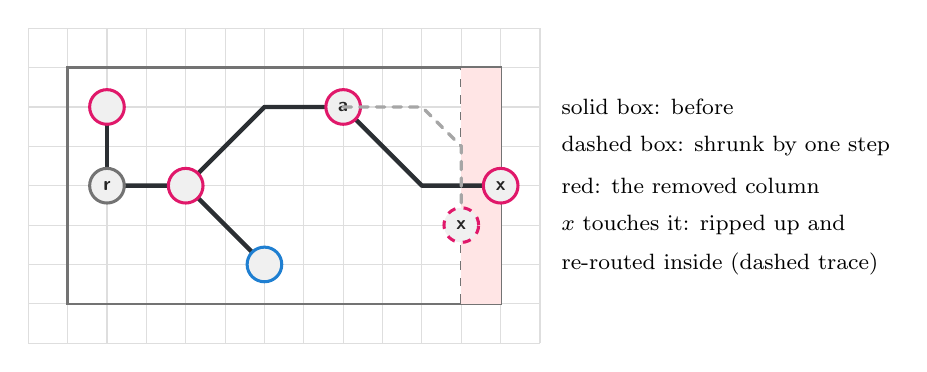
\begin{tikzpicture}[x=0.5cm,y=-0.5cm]
  \gridbg{0}{0}{13}{8}
  \draw[black!55,line width=0.8pt] (1,1) rectangle (12,7);
  \draw[black!55,line width=0.8pt,dashed] (1,1) rectangle (11,7);
  \fill[red!10] (11,1) rectangle (12,7);
  \draw[trace] (2,4)--(4,4)--(6,2)--(8,2); \draw[trace] (4,4)--(6,6); \draw[trace] (2,4)--(2,2);
  \draw[trace] (8,2)--(10,4)--(12,4);
  \node[npad] at (2,4){r}; \node[fpad] at (4,4){}; \node[fpad] at (8,2){a}; \node[mpad] at (6,6){}; \node[fpad] at (2,2){};
  \node[fpad] at (12,4){x};
  \draw[ghost] (8,2)--(10,2)--(11,3)--(11,5);
  \node[pad,draw=femalec,dashed] at (11,5){x};
  \node[font=\footnotesize,anchor=west] at (13.3,2){solid box: before};
  \node[font=\footnotesize,anchor=west] at (13.3,3){dashed box: shrunk by one step};
  \node[font=\footnotesize,anchor=west] at (13.3,4){red: the removed column};
  \node[font=\footnotesize,anchor=west] at (13.3,5){$x$ touches it: ripped up and};
  \node[font=\footnotesize,anchor=west] at (13.3,6){re-routed inside (dashed trace)};
\end{tikzpicture}
\caption{One squeeze step on the right side. The sub-tree of $x$ is the only one touching the right column; it is
routed again inside the box shrunk by one column, here with a chamfered corner.}
\label{fig:squeeze}
\end{figure}

%=====================================================================================================================
\section{Forest packing}\label{sec:packing}

\subsection{Tree classes}
The trees of the forest are split by their number of vertices $n_T$ into \emph{large} ($n_T\ge 9$),
\emph{medium} ($4\le n_T\le 8$) and \emph{small} ($n_T\le 3$) trees. Large and medium trees are routed as in
Section~\ref{sec:routing}; the time budgets of the squeeze and of the extra attempts are shared by these trees only,
in proportion to their size. Small trees are not routed at all: their drawings come from templates
(Section~\ref{sec:templates}) and cost $O(1)$ time each.

\subsection{Straight templates for small trees}\label{sec:templates}

A small tree is an isolated vertex, a single edge, or a path $x$--$y$--$z$. Its \emph{variants} are all drawings in
which every edge is one straight trace: from the parent the trace runs in a direction whose parity matches the gender
of the child (orthogonal into a female, diagonal into a male), with length $c$, or, for a single edge only, also $c+1$.
Every vertex may be the root (or only the user's root node, if it lies in this tree). Each variant has a \emph{rank},
its total extra length ($0$ for the shortest traces). Variants with the same geometry (labels ignored, after
translation) are merged, keeping the lowest rank; a single edge has $4$ variants, a path of three vertices at most
$48$ (Figure~\ref{fig:templates}).

\begin{proposition}\label{prop:straight}
Every small tree has a valid drawing with only straight traces of length $c$ that obeys the gender rule, for any
choice of root. In particular a tree of two vertices is always drawn as one straight trace without bends.
\end{proposition}
\begin{proof}
For a single edge $r\to s$ choose any direction $D_k$ whose parity matches $g(s)$ and put $\pos(s)=\pos(r)+cD_k$; the
two pads are at distance $c$ and the trace has no other trace to meet. For a path rooted at its middle $y$, choose
directions $D_a\ne D_b$ with the parities required by the two ends; the rays meet only in $y$, and since $D_a$ and
$D_b$ differ by at least $1$ in some coordinate, the end pads are at Chebyshev distance at least $c$. For a path
rooted at an end, $x\to y$ in $D_a$ and $y\to z$ in $D_b\ne -D_a$ (four choices of $D_b$ remain); then
$\pos(z)-\pos(x)=c(D_a+D_b)$ has a coordinate of absolute value at least $c$ because $D_a+D_b\ne 0$, the two rays share
only $y$, and their diagonal steps at $y$ lie in different unit squares (that would need $D_b=-D_a$).
\end{proof}

\begin{figure}[t]
\centering
\begin{subfigure}[b]{0.23\textwidth}\centering
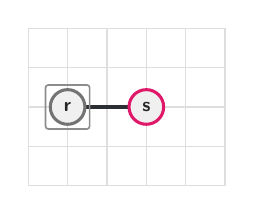
\begin{tikzpicture}[x=0.5cm,y=-0.5cm]
  \gridbg{0}{0}{5}{4}
  \draw[trace] (1,2)--(3,2);
  \node[rootbox] at (1,2){}; \node[npad] at (1,2){r}; \node[fpad] at (3,2){s};
\end{tikzpicture}
\caption{Edge, female child: one straight trace.}
\end{subfigure}\hfill
\begin{subfigure}[b]{0.23\textwidth}\centering
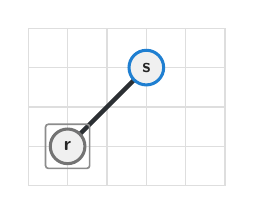
\begin{tikzpicture}[x=0.5cm,y=-0.5cm]
  \gridbg{0}{0}{5}{4}
  \draw[trace] (1,3)--(3,1);
  \node[rootbox] at (1,3){}; \node[npad] at (1,3){r}; \node[mpad] at (3,1){s};
\end{tikzpicture}
\caption{Edge, male child: one straight diagonal.}
\end{subfigure}\hfill
\begin{subfigure}[b]{0.23\textwidth}\centering
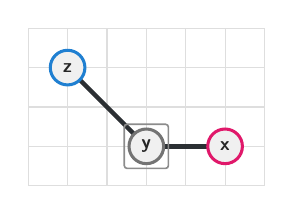
\begin{tikzpicture}[x=0.5cm,y=-0.5cm]
  \gridbg{-1}{-1}{5}{3}
  \draw[trace] (2,2)--(4,2); \draw[trace] (2,2)--(0,0);
  \node[rootbox] at (2,2){}; \node[npad] at (2,2){y}; \node[fpad] at (4,2){x}; \node[mpad] at (0,0){z};
\end{tikzpicture}
\caption{Path rooted at its middle.}
\end{subfigure}\hfill
\begin{subfigure}[b]{0.23\textwidth}\centering
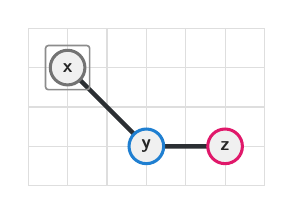
\begin{tikzpicture}[x=0.5cm,y=-0.5cm]
  \gridbg{-1}{-1}{5}{3}
  \draw[trace] (0,0)--(2,2)--(4,2);
  \node[rootbox] at (0,0){}; \node[npad] at (0,0){x}; \node[mpad] at (2,2){y}; \node[fpad] at (4,2){z};
\end{tikzpicture}
\caption{Path rooted at an end.}
\end{subfigure}
\caption{Straight-only templates of small trees (framed: root). Each edge is one straight trace of length $c=2$ whose
direction follows the gender of the child; no template contains a bend. A single edge also has variants of length
$c+1$ (rank $1$), used only if no shortest one fits.}
\label{fig:templates}
\end{figure}

\subsection{Rotations and reflections}
\begin{lemma}\label{lem:d8}
Let $g$ be one of the eight symmetries of the grid (rotations by multiples of $90^\circ$ and reflections in the axes
and diagonals). Applying $g$ to all pads and traces of a valid drawing gives a valid drawing that obeys the gender rule.
\end{lemma}
\begin{proof}
$g$ is an integer orthogonal map: it maps grid points bijectively to grid points, preserves Chebyshev distances
(so \ref{c:pad} holds), maps unit octilinear steps to unit octilinear steps, orthogonal ones to orthogonal ones and
diagonal ones to diagonal ones (so \ref{c:gender} holds), keeps distinct points distinct (\ref{c:excl}), and maps the
two diagonals of a unit square to the two diagonals of the image square (\ref{c:diag}).
\end{proof}
Every routed tree therefore has up to eight \emph{variants} for free (duplicates of symmetric drawings are removed).

\subsection{The board grid}
Packing works on one board stored as flat typed arrays over a rectangle of grid points that grows on demand (by at
least $32$ steps per side, copying row by row): \texttt{occ} marks occupied points (pads and trace points),
\texttt{pz} the \emph{pad zone} (points closer than $c$ to a placed pad), \texttt{dg} the used diagonal slots of every
unit square, and \texttt{near}$(q)$ the number of occupied points within Chebyshev distance $2$ of $q$. A variant is
stored as its \emph{footprint}: the lists of its pads, of all its points, and of its diagonal slots. A placement at
offset $o$ is \emph{legal} if no pad of the footprint lies in the pad zone, no point is occupied and no diagonal
crosses a used one; each test is one array lookup, so a legality check costs $O(|\text{footprint}|)$. Cells outside
the allocated rectangle are empty.

\begin{proposition}
Every packed board satisfies \ref{c:pad}--\ref{c:gender}.
\end{proposition}
\begin{proof}
Inside a tree the constraints hold by construction (Sections~\ref{sec:routing} and~\ref{sec:templates}) and are
preserved by translation and, by Lemma~\ref{lem:d8}, by the symmetries. Between trees, a legal placement has no pad
closer than $c$ to another tree's pad, no point in common with another tree, and no crossing diagonals, which are
exactly \ref{c:pad}--\ref{c:diag}.
\end{proof}

\subsection{Order and score}
The largest tree (by footprint size) is placed first, in its original orientation. Then come the other large trees,
then the medium trees, then the small trees by decreasing size ($3$, $2$, $1$). For a placement that turns the board
box $B$ into $B'$ of $W\times H$ steps, the score is lexicographic, smaller first:
\[
\bigl(\,f(B')=\max(W,\ \alpha H),\ \ (W+1)(H+1),\ \ \text{rank},\ \ -\mathrm{contact}\,\bigr),
\]
where $\alpha$ is the board aspect (width/height, default $1.6$) and
$\mathrm{contact}=\sum_{q\in\text{footprint}}\min(\texttt{near}(q),4)$ measures how snugly the variant sits against what
is already drawn. Rank and contact are used only for medium and small trees (\emph{nestling}); for large trees, ties
keep the scan order.

\paragraph{Large trees.} All variants and all offsets that keep the tree within distance $c$ of the board are
scanned; a candidate is tested for legality only if its $(f,\text{area})$ could beat the best one found so far.

\subsection{Nestling medium and small trees}\label{sec:nestle}

A variant can only be placed where its first pad lands on a free cell (not occupied and outside every pad zone). The
search is therefore driven by free cells instead of all offsets, in two passes (Figure~\ref{fig:nestle},
Algorithm~\ref{alg:nestle}):
\begin{enumerate}[nosep]
  \item \textbf{Inside.} The free cells inside $B$ are listed once; every variant is anchored on each of them and kept
        if it lies completely inside $B$ and is legal. The board does not grow, so the best candidate has the lowest
        rank and, among those, the most contact. If there is one, it is taken.
  \item \textbf{Grow.} Otherwise the board must grow. The boxes $B$ pushed out by $k=1,2,\dots,e+c+1$ steps on one side
        ($e$ = the largest variant extent) are sorted by $(f,\text{area})$. In each box only anchors in the new strip
        and within distance $e$ of it are tried, and only placements that reach into the strip (all others failed in
        pass 1). The first box with a legal placement decides; in it, rank and then contact pick the winner.
\end{enumerate}
Pass 2 makes the next small trees cheap again: they find room in the new strip during pass 1. Because the shortest
variants have rank $0$, a single edge uses its longer variant only when no shortest one fits anywhere in the board;
in all tests every single edge was drawn at length $c$.

\begin{figure}[t]
\centering
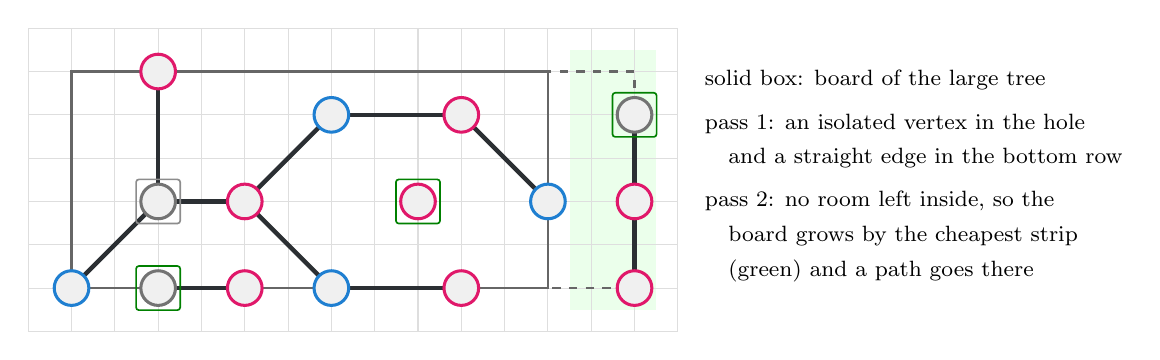
\begin{tikzpicture}[x=0.55cm,y=-0.55cm]
  \fill[green!8] (12.5,0.5) rectangle (14.5,6.5);
  \gridbg{0}{0}{15}{7}
  \draw[black!60,line width=0.8pt] (1,1) rectangle (12,6);
  \draw[black!60,line width=0.8pt,dashed] (1,1) rectangle (14,6);
  % large tree
  \draw[trace] (3,4)--(5,4); \draw[trace] (5,4)--(7,2); \draw[trace] (7,2)--(10,2); \draw[trace] (5,4)--(7,6);
  \draw[trace] (7,6)--(10,6); \draw[trace] (3,4)--(3,1); \draw[trace] (3,4)--(1,6); \draw[trace] (10,2)--(12,4);
  \node[rootbox] at (3,4){};
  \node[npad] at (3,4){}; \node[fpad] at (5,4){}; \node[mpad] at (7,2){}; \node[fpad] at (10,2){};
  \node[mpad] at (7,6){}; \node[fpad] at (10,6){}; \node[fpad] at (3,1){}; \node[mpad] at (1,6){}; \node[mpad] at (12,4){};
  % nestled small trees
  \node[rootbox,draw=green!50!black] at (9,4){}; \node[fpad] at (9,4){};
  \draw[trace] (3,6)--(5,6); \node[rootbox,draw=green!50!black] at (3,6){}; \node[npad] at (3,6){}; \node[fpad] at (5,6){};
  \draw[trace] (14,2)--(14,6); \node[rootbox,draw=green!50!black] at (14,2){}; \node[npad] at (14,2){}; \node[fpad] at (14,4){}; \node[fpad] at (14,6){};
  \node[font=\footnotesize,anchor=west] at (15.4,1.2) {solid box: board of the large tree};
  \node[font=\footnotesize,anchor=west] at (15.4,2.2) {pass 1: an isolated vertex in the hole};
  \node[font=\footnotesize,anchor=west] at (15.4,3.0) {\quad and a straight edge in the bottom row};
  \node[font=\footnotesize,anchor=west] at (15.4,4.0) {pass 2: no room left inside, so the};
  \node[font=\footnotesize,anchor=west] at (15.4,4.8) {\quad board grows by the cheapest strip};
  \node[font=\footnotesize,anchor=west] at (15.4,5.6) {\quad (green) and a path goes there};
\end{tikzpicture}
\caption{Nestling. Small trees (green frames: their roots) are placed into free cells inside the board first; only
when none fits does the board grow, by the strip that enlarges it least.}
\label{fig:nestle}
\end{figure}

\begin{algorithm}[t]
\caption{\textsc{Nestle}$(\text{variants } V)$ --- placement of a medium or small tree}\label{alg:nestle}
\DontPrintSemicolon
$F_{\mathrm{in}}\gets$ free cells inside $B$;\quad $\mathit{best}\gets$ none\;
\ForEach{$v\in V$, $q\in F_{\mathrm{in}}$}{
  $o\gets q-\text{first pad of } v$\;
  \If{$v+o\subseteq B$ \textbf{and} legal$(v,o)$}{keep $(v,o)$ if better by (rank, $-$contact)}
}
\lIf{$\mathit{best}$}{\KwRet{$\mathit{best}$}}
\ForEach{box $B'$ = $B$ pushed out by $k$ on one side, by increasing $(f(B'),\text{area})$}{
  \lIf{$\mathit{best}$ \textbf{and} $B'$ is worse than $\mathit{best}$}{\Break}
  \ForEach{$v\in V$, free anchor $q$ in the strip of $B'$ (or within distance $e$ of it)}{
    $o\gets q-\text{first pad of } v$\;
    \If{$v+o\subseteq B'$, $v+o\not\subseteq B$ \textbf{and} legal$(v,o)$}{keep $(v,o)$ if better by (rank, $-$contact)}
  }
}
\KwRet{$\mathit{best}$}
\end{algorithm}

Finally the board is translated so that its box starts at $(1,1)$, leaving a margin of one grid step.

%=====================================================================================================================
\section{Verification}\label{sec:verify}

After packing, the drawing is checked by a procedure that shares no data with the construction. It re-derives
everything from the final coordinates:
\begin{enumerate}[nosep]
  \item \textbf{Pads}: two pads on the same point; every pair of pads closer than $c$ (all pairs, $O(n^2)$).
  \item \textbf{Traces}: start and end on the pads of the edge; every step is a unit octilinear step; no interior
        point is a pad; no interior point is used by two traces (overlap); no unit square contains both diagonals
        (crossing).
  \item \textbf{Gender}: the last step of the trace to $v$ is diagonal iff $g(v)=\mathrm M$.
\end{enumerate}
Problems are listed in three reports and circled in the drawing. By the construction rules, a layout without forced
routes passes all checks, and by Proposition~\ref{prop:planar} it is crossing-free. Because all coordinates are
integers, the checks are exact.

%=====================================================================================================================
\section{Running time}\label{sec:complexity}

\paragraph{Enumeration.} Let $n$ be the number of vertices of a routed tree and $L$ the maximum segment length. The
enumeration for one child visits at most $8L$ straight, $16L^2$ one-bend and $96L^2$ two-bend candidates (middle
segment $\le3$, dogleg or chamfered corner). Extending a path costs $O(L)$ for the self-intersection test plus
$O(1)$ for the reservation and the bus bonus, so the first stage costs $O(L^3)$ per child and $O(nL^3)$ per tree. The
second stage ($2L$) multiplies this by a constant. The maze router is bounded by $60\,000$ expansions of five moves
each; rip-up repeats \textsc{FindRoute} at most $\sum_{m=1}^{6}(m+1)=27$ times for a failing child. Multi-start and
squeeze are bounded by their time budgets.

The following three speed-ups change \emph{no} drawing (checked on random trees: identical pads and traces), but
make the routing about six times faster in practice.

\paragraph{1. Branch and bound.} Let $G$ be the bus bonus collected so far. For a partial trace with length $\ell$,
$b$ bends and box growth $\Delta H$, the cost of every completion satisfies
\[
C(\pi)\ \ge\ \underline{C}=\ell-\sigma G+0.7\,b+\lambda\,\Delta H-1,
\]
because all look-ahead terms are non-negative and the continuation bonus is at most $1$.
\begin{proposition}
If $\sigma\le 1$ and $\omega=0$ (the defaults), $\underline C$ never decreases when the partial trace is extended.
Hence a walk can be stopped as soon as $\underline C\ge C(\pi^\ast)$ for the best candidate $\pi^\ast$ found so far,
without changing the result.
\end{proposition}
\begin{proof}
An extra step adds its length ($1$ or $\sqrt 2$) to $\ell$ and at most $\sigma\le1$ to $\sigma G$, so
$\ell-\sigma G$ does not decrease; $b$ and $\Delta H$ (the box only grows) do not decrease either. Every completion of a
stopped walk therefore costs at least $C(\pi^\ast)$ and cannot replace $\pi^\ast$, which wins ties as the first one
found.
\end{proof}
For other settings (the radial variant of the multi-start, or $\sigma>1$) the test is switched off.

\paragraph{2. Reservation table.} Instead of scanning the $5\times5$ window around every step for waiting pads
(Section~\ref{sec:legal}), the waiting pads are entered once per child into two tables, \emph{near} (distance $1$) and
\emph{ring} (distance $2$, without $u$), keyed by grid point. A step then needs one lookup. Building the tables costs
$24$ entries per waiting pad.

\paragraph{3. Lazy look-ahead cache.} The free directions and the free room around an end point depend only on the
committed drawing, so they are computed once per end point and child, and only for candidates that pass the lower
bound. The diagonal slots are computed without allocating objects.

\paragraph{Packing.} A small tree has at most $48$ variants with at most $5$ footprint points. Pass 1 costs
$O(|F_{\mathrm{in}}|\cdot|V|)$ legality checks of constant size, where $|F_{\mathrm{in}}|$ is the number of free cells
inside the board, which shrinks as the board fills; pass 2 examines one or two strips in practice. With
$|B|$ the number of board cells, packing $k_s$ small trees costs $O(k_s\,|B|)$ in the worst case, against
$O(k_s\,|B|\,|V|)$ for a scan over all offsets. Placing a large tree costs $O(8\,|B|\,|\text{footprint}|)$ in the
worst case. Verification costs $O(n^2+\sum_e|\pi(e)|)$.

%=====================================================================================================================
\section{Results}\label{sec:experiments}

All measurements use the default settings ($L=6$, $c=2$, $\lambda=1.5$, $\sigma=0.5$, $\alpha=1.6$, BFS order,
two-bend traces and squeeze on, $T_{\mathrm{squeeze}}=800$\,ms, $T_{\mathrm{choose}}=0$) and run the unchanged
JavaScript of the page \texttt{electric\_map.html} in Node.js~22, single-threaded. Board sizes count grid steps; ``points per
vertex'' is the number of grid points of the board box divided by the number of vertices.

\paragraph{Examples.} Figure~\ref{fig:example1} shows a forest of three trees (21 vertices, 18 edges) and
Figure~\ref{fig:example2} a forest of the target kind with $100$ vertices: three large trees, one medium tree and $21$
small trees. Both are drawn here from the computed coordinates. Note the straight single edges and paths nestled
around the large trees, the chamfered corners, and the parallel runs on adjacent grid lines.

\begin{figure}[p]
\centering
\begin{minipage}{0.28\textwidth}
\begin{lstlisting}[basicstyle=\ttfamily\footnotesize]
*A:B,*C,D
B:*A,*E,F,G
*C:*A,H,*I
D:*A,*J
*E:B,K,*L
F:B
G:B,*M
H:*C
*I:*C,N,*O
*J:D
K:*E
*L:*E
*M:G
N:*I
*O:*I
P:*Q,R,*S
*Q:P
R:P,*T
*S:P
*T:R
U:
\end{lstlisting}
\end{minipage}\hfill
\begin{minipage}{0.68\textwidth}\centering
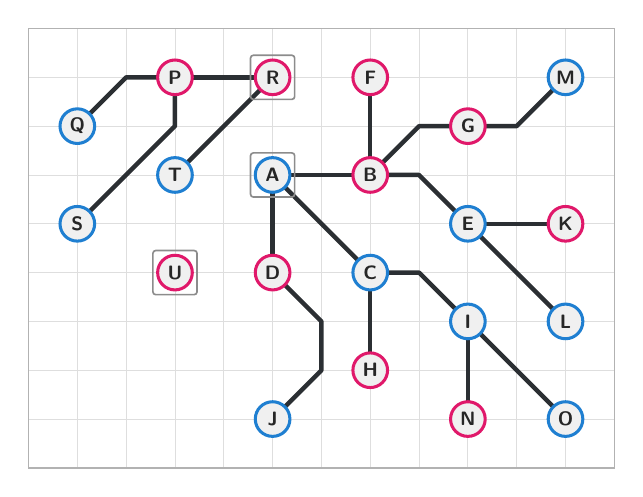
\begin{tikzpicture}[x=0.62cm,y=-0.62cm]
\draw[gridc,line width=0.3pt,step={(1,-1)}] (0,0) grid (12,9);
\draw[gray!60,line width=0.6pt] (0,0) rectangle (12,9);
\draw[trace] (5,3) -- (7,3);
\draw[trace] (5,3) -- (7,5);
\draw[trace] (5,3) -- (5,5);
\draw[trace] (7,3) -- (8,3) -- (9,4);
\draw[trace] (7,3) -- (8,2) -- (9,2);
\draw[trace] (7,3) -- (7,1);
\draw[trace] (7,5) -- (8,5) -- (9,6);
\draw[trace] (7,5) -- (7,7);
\draw[trace] (9,4) -- (11,4);
\draw[trace] (9,4) -- (11,6);
\draw[trace] (9,2) -- (10,2) -- (11,1);
\draw[trace] (9,6) -- (9,8);
\draw[trace] (9,6) -- (11,8);
\draw[trace] (5,5) -- (6,6) -- (6,7) -- (5,8);
\draw[trace] (5,1) -- (3,1);
\draw[trace] (5,1) -- (3,3);
\draw[trace] (3,1) -- (2,1) -- (1,2);
\draw[trace] (3,1) -- (3,2) -- (1,4);
\node[rootbox] at (5,3) {};
\node[mpad] at (5,3) {A};
\node[fpad] at (7,3) {B};
\node[mpad] at (7,5) {C};
\node[fpad] at (5,5) {D};
\node[mpad] at (9,4) {E};
\node[fpad] at (9,2) {G};
\node[fpad] at (7,1) {F};
\node[mpad] at (9,6) {I};
\node[fpad] at (7,7) {H};
\node[fpad] at (11,4) {K};
\node[mpad] at (11,6) {L};
\node[mpad] at (11,1) {M};
\node[fpad] at (9,8) {N};
\node[mpad] at (11,8) {O};
\node[mpad] at (5,8) {J};
\node[rootbox] at (5,1) {};
\node[fpad] at (5,1) {R};
\node[fpad] at (3,1) {P};
\node[mpad] at (3,3) {T};
\node[mpad] at (1,2) {Q};
\node[mpad] at (1,4) {S};
\node[rootbox] at (3,5) {};
\node[fpad] at (3,5) {U};
\end{tikzpicture}
\end{minipage}
\caption{Input (left) and computed board (right) of a forest of three trees: $10\times7$ grid, $4.2$ grid points per
vertex, average trace length $2.50$ steps, $11$ of $18$ traces straight, no conflicts. Framed pads are the roots;
$U$ is an isolated vertex.}
\label{fig:example1}

\vspace{8mm}
\begingroup
\tikzset{pad/.append style={minimum size=3.6mm,font=\sffamily\bfseries\tiny},rootbox/.append style={minimum size=4.6mm}}
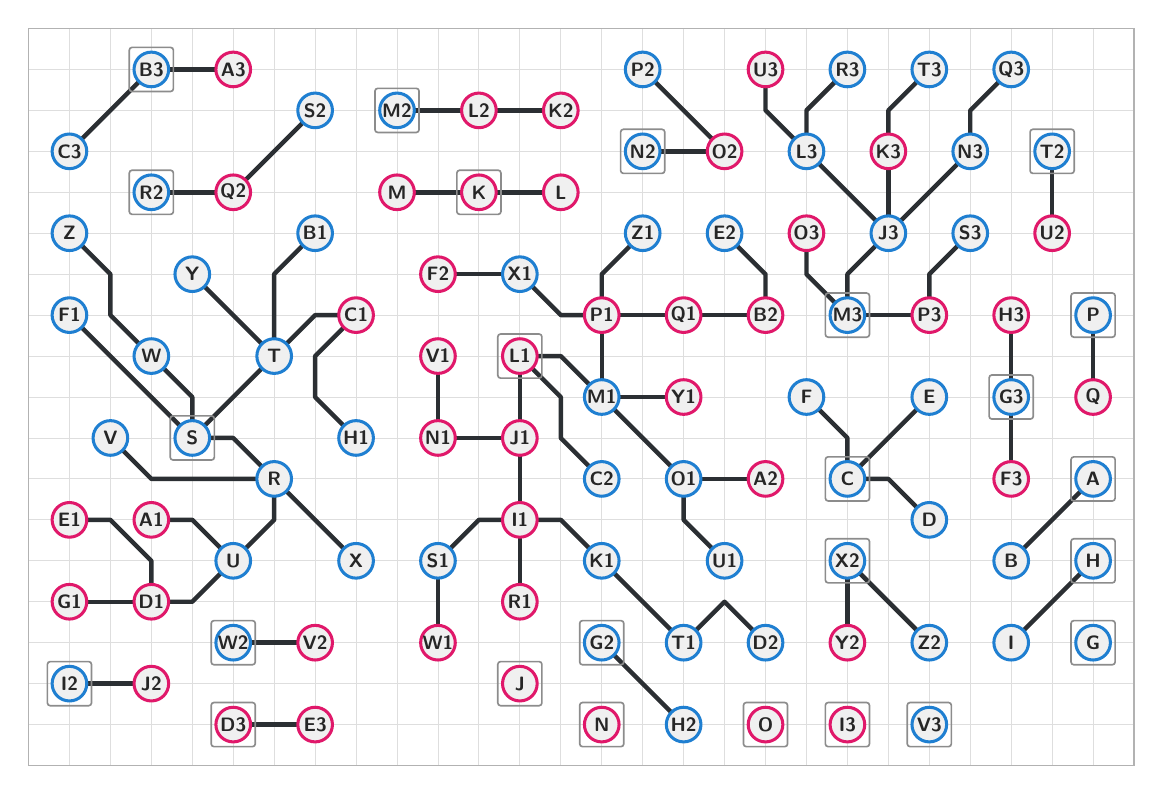
\begin{tikzpicture}[x=0.52cm,y=-0.52cm]
\draw[gridc,line width=0.3pt,step={(1,-1)}] (0,0) grid (27,18);
\draw[gray!60,line width=0.6pt] (0,0) rectangle (27,18);
\draw[trace] (26,11) -- (24,13);
\draw[trace] (20,11) -- (21,11) -- (22,12);
\draw[trace] (20,11) -- (22,9);
\draw[trace] (20,11) -- (20,10) -- (19,9);
\draw[trace] (26,13) -- (24,15);
\draw[trace] (11,4) -- (13,4);
\draw[trace] (11,4) -- (9,4);
\draw[trace] (26,7) -- (26,9);
\draw[trace] (4,10) -- (5,10) -- (6,11);
\draw[trace] (4,10) -- (6,8);
\draw[trace] (4,10) -- (4,9) -- (3,8);
\draw[trace] (6,11) -- (6,12) -- (5,13);
\draw[trace] (6,8) -- (7,7) -- (8,7);
\draw[trace] (6,8) -- (4,6);
\draw[trace] (6,8) -- (6,6) -- (7,5);
\draw[trace] (5,13) -- (4,14) -- (3,14);
\draw[trace] (8,7) -- (7,8) -- (7,9) -- (8,10);
\draw[trace] (3,14) -- (1,14);
\draw[trace] (6,11) -- (8,13);
\draw[trace] (4,10) -- (1,7);
\draw[trace] (6,11) -- (3,11) -- (2,10);
\draw[trace] (3,8) -- (2,7) -- (2,6) -- (1,5);
\draw[trace] (5,13) -- (4,12) -- (3,12);
\draw[trace] (3,14) -- (3,13) -- (2,12) -- (1,12);
\draw[trace] (12,8) -- (13,8) -- (14,9);
\draw[trace] (12,8) -- (12,10);
\draw[trace] (12,8) -- (13,9) -- (13,10) -- (14,11);
\draw[trace] (12,10) -- (12,12);
\draw[trace] (12,10) -- (10,10);
\draw[trace] (14,9) -- (14,7);
\draw[trace] (14,9) -- (16,11);
\draw[trace] (14,9) -- (16,9);
\draw[trace] (12,12) -- (13,12) -- (14,13);
\draw[trace] (12,12) -- (11,12) -- (10,13);
\draw[trace] (12,12) -- (12,14);
\draw[trace] (10,10) -- (10,8);
\draw[trace] (16,11) -- (16,12) -- (17,13);
\draw[trace] (16,11) -- (18,11);
\draw[trace] (14,7) -- (16,7);
\draw[trace] (14,7) -- (13,7) -- (12,6);
\draw[trace] (14,7) -- (14,6) -- (15,5);
\draw[trace] (14,13) -- (16,15);
\draw[trace] (10,13) -- (10,15);
\draw[trace] (16,7) -- (18,7);
\draw[trace] (12,6) -- (10,6);
\draw[trace] (18,7) -- (18,6) -- (17,5);
\draw[trace] (16,15) -- (17,14) -- (18,15);
\draw[trace] (14,15) -- (16,17);
\draw[trace] (1,16) -- (3,16);
\draw[trace] (9,2) -- (11,2);
\draw[trace] (11,2) -- (13,2);
\draw[trace] (15,3) -- (17,3);
\draw[trace] (17,3) -- (15,1);
\draw[trace] (3,4) -- (5,4);
\draw[trace] (5,4) -- (7,2);
\draw[trace] (25,3) -- (25,5);
\draw[trace] (5,15) -- (7,15);
\draw[trace] (20,13) -- (20,15);
\draw[trace] (20,13) -- (22,15);
\draw[trace] (3,1) -- (5,1);
\draw[trace] (3,1) -- (1,3);
\draw[trace] (5,17) -- (7,17);
\draw[trace] (24,9) -- (24,11);
\draw[trace] (24,9) -- (24,7);
\draw[trace] (20,7) -- (20,6) -- (21,5);
\draw[trace] (20,7) -- (22,7);
\draw[trace] (20,7) -- (19,6) -- (19,5);
\draw[trace] (21,5) -- (19,3);
\draw[trace] (21,5) -- (21,3);
\draw[trace] (21,5) -- (23,3);
\draw[trace] (22,7) -- (22,6) -- (23,5);
\draw[trace] (21,3) -- (21,2) -- (22,1);
\draw[trace] (19,3) -- (19,2) -- (20,1);
\draw[trace] (19,3) -- (18,2) -- (18,1);
\draw[trace] (23,3) -- (23,2) -- (24,1);
\node[rootbox] at (26,11) {};
\node[mpad] at (26,11) {A};
\node[mpad] at (24,13) {B};
\node[rootbox] at (20,11) {};
\node[mpad] at (20,11) {C};
\node[mpad] at (22,12) {D};
\node[mpad] at (22,9) {E};
\node[mpad] at (19,9) {F};
\node[rootbox] at (26,15) {};
\node[mpad] at (26,15) {G};
\node[rootbox] at (26,13) {};
\node[mpad] at (26,13) {H};
\node[mpad] at (24,15) {I};
\node[rootbox] at (12,16) {};
\node[fpad] at (12,16) {J};
\node[rootbox] at (11,4) {};
\node[fpad] at (11,4) {K};
\node[fpad] at (13,4) {L};
\node[fpad] at (9,4) {M};
\node[rootbox] at (14,17) {};
\node[fpad] at (14,17) {N};
\node[rootbox] at (18,17) {};
\node[fpad] at (18,17) {O};
\node[rootbox] at (26,7) {};
\node[mpad] at (26,7) {P};
\node[fpad] at (26,9) {Q};
\node[rootbox] at (4,10) {};
\node[mpad] at (4,10) {S};
\node[mpad] at (6,11) {R};
\node[mpad] at (6,8) {T};
\node[mpad] at (3,8) {W};
\node[mpad] at (5,13) {U};
\node[fpad] at (8,7) {C1};
\node[mpad] at (4,6) {Y};
\node[mpad] at (7,5) {B1};
\node[fpad] at (3,14) {D1};
\node[mpad] at (8,10) {H1};
\node[fpad] at (1,14) {G1};
\node[mpad] at (8,13) {X};
\node[mpad] at (1,7) {F1};
\node[mpad] at (2,10) {V};
\node[mpad] at (1,5) {Z};
\node[fpad] at (3,12) {A1};
\node[fpad] at (1,12) {E1};
\node[rootbox] at (12,8) {};
\node[fpad] at (12,8) {L1};
\node[mpad] at (14,9) {M1};
\node[fpad] at (12,10) {J1};
\node[mpad] at (14,11) {C2};
\node[fpad] at (12,12) {I1};
\node[fpad] at (10,10) {N1};
\node[fpad] at (14,7) {P1};
\node[mpad] at (16,11) {O1};
\node[fpad] at (16,9) {Y1};
\node[mpad] at (14,13) {K1};
\node[mpad] at (10,13) {S1};
\node[fpad] at (12,14) {R1};
\node[fpad] at (10,8) {V1};
\node[mpad] at (17,13) {U1};
\node[fpad] at (18,11) {A2};
\node[fpad] at (16,7) {Q1};
\node[mpad] at (12,6) {X1};
\node[mpad] at (15,5) {Z1};
\node[mpad] at (16,15) {T1};
\node[fpad] at (10,15) {W1};
\node[fpad] at (18,7) {B2};
\node[fpad] at (10,6) {F2};
\node[mpad] at (17,5) {E2};
\node[mpad] at (18,15) {D2};
\node[rootbox] at (14,15) {};
\node[mpad] at (14,15) {G2};
\node[mpad] at (16,17) {H2};
\node[rootbox] at (1,16) {};
\node[mpad] at (1,16) {I2};
\node[fpad] at (3,16) {J2};
\node[rootbox] at (9,2) {};
\node[mpad] at (9,2) {M2};
\node[fpad] at (11,2) {L2};
\node[fpad] at (13,2) {K2};
\node[rootbox] at (15,3) {};
\node[mpad] at (15,3) {N2};
\node[fpad] at (17,3) {O2};
\node[mpad] at (15,1) {P2};
\node[rootbox] at (3,4) {};
\node[mpad] at (3,4) {R2};
\node[fpad] at (5,4) {Q2};
\node[mpad] at (7,2) {S2};
\node[rootbox] at (25,3) {};
\node[mpad] at (25,3) {T2};
\node[fpad] at (25,5) {U2};
\node[rootbox] at (5,15) {};
\node[mpad] at (5,15) {W2};
\node[fpad] at (7,15) {V2};
\node[rootbox] at (20,13) {};
\node[mpad] at (20,13) {X2};
\node[fpad] at (20,15) {Y2};
\node[mpad] at (22,15) {Z2};
\node[rootbox] at (3,1) {};
\node[mpad] at (3,1) {B3};
\node[fpad] at (5,1) {A3};
\node[mpad] at (1,3) {C3};
\node[rootbox] at (5,17) {};
\node[fpad] at (5,17) {D3};
\node[fpad] at (7,17) {E3};
\node[rootbox] at (24,9) {};
\node[mpad] at (24,9) {G3};
\node[fpad] at (24,11) {F3};
\node[fpad] at (24,7) {H3};
\node[rootbox] at (20,17) {};
\node[fpad] at (20,17) {I3};
\node[rootbox] at (20,7) {};
\node[mpad] at (20,7) {M3};
\node[mpad] at (21,5) {J3};
\node[fpad] at (22,7) {P3};
\node[fpad] at (19,5) {O3};
\node[mpad] at (19,3) {L3};
\node[fpad] at (21,3) {K3};
\node[mpad] at (23,3) {N3};
\node[mpad] at (23,5) {S3};
\node[mpad] at (22,1) {T3};
\node[mpad] at (20,1) {R3};
\node[fpad] at (18,1) {U3};
\node[mpad] at (24,1) {Q3};
\node[rootbox] at (22,17) {};
\node[mpad] at (22,17) {V3};
\end{tikzpicture}
\endgroup
\caption{The test forest with $100$ vertices (\texttt{forest\_100.txt}: large trees of $24$, $17$ and $12$ vertices,
a medium tree of $4$, and $21$ small trees): $25\times16$ grid, $4.4$ grid points per vertex, all $8$ single edges
straight at the shortest length, no conflicts, under $0.3$\,s.}
\label{fig:example2}
\end{figure}

\paragraph{Single large trees.} Table~\ref{tab:results} reports random recursive trees (vertex $i$ attaches to a
random earlier vertex whose degree is below a cap $\Delta$) with random genders, six instances per row. Time includes
the multi-start, so rows with forced routes use the $4$-second retry budget.

\begin{table}[t]
\centering
\caption{Random single trees (6 instances per row, averages unless stated).}
\label{tab:results}
\small\setlength{\tabcolsep}{4.2pt}
\begin{tabular}{rrcrrrrrrr}
\toprule
$n$ & $\Delta$ & conflict- & points per & trace & straight & two-bend & steps & forced & time\\
 & & free & vertex & length & & & in buses & (sum) & [ms]\\
\midrule
25 & 4 & 6/6 & 4.57 & 2.78 & 56\% & 8.3\% & 14\% & 0 & 60\\
50 & 4 & 6/6 & 5.06 & 2.92 & 50\% & 8.8\% & 22\% & 0 & 87\\
100 & 4 & 6/6 & 5.57 & 3.11 & 52\% & 6.4\% & 31\% & 0 & 649\\
200 & 4 & 0/6 & 6.47 & 3.67 & 45\% & 9.9\% & 43\% & 86 & 5268\\
100 & 6 & 5/6 & 5.71 & 3.38 & 46\% & 7.6\% & 36\% & 1 & 2006\\
\bottomrule
\end{tabular}
\end{table}

\paragraph{Target forests.} Table~\ref{tab:forests} compares the five test forests (100--300 vertices) laid out by
the general version of the algorithm (every tree routed, packing by bounding-box footprint without symmetries or
nestling) and by the specialised one described here. On a wider set of $28$ random forests of the same kind (1--5
large trees, up to $90$ small trees, up to $2$ medium trees), the specialised version needs $4.6\%$ less board area
in total (smaller in $21$ forests, larger in $2$), is $5.0$ times faster ($20.1$\,s against $4.1$\,s in total), and
draws no single edge with a bend, against $190$ bent single edges before. No layout had any conflict.

\begin{table}[t]
\centering
\caption{The five test forests (L/M/S = large/medium/small trees; bent = single edges drawn with a bend / all single
edges).}
\label{tab:forests}
\small\setlength{\tabcolsep}{3.6pt}
\begin{tabular}{rrc|rrrr|rrrr}
\toprule
 & & & \multicolumn{4}{c|}{general version} & \multicolumn{4}{c}{specialised version}\\
$n$ & trees & L/M/S & board & pts/vertex & bent & ms & board & pts/vertex & bent & ms\\
\midrule
100 & 25 & 3/1/21 & $27\times16$ & 4.76 & 4/8 & 703 & $25\times16$ & 4.42 & 0/8 & 272 \\
150 & 31 & 4/1/26 & $32\times20$ & 4.62 & 4/7 & 764 & $32\times20$ & 4.62 & 0/7 & 137 \\
200 & 45 & 5/2/38 & $38\times23$ & 4.68 & 9/13 & 1176 & $37\times23$ & 4.56 & 0/13 & 348 \\
250 & 60 & 5/1/54 & $42\times26$ & 4.64 & 10/18 & 1152 & $41\times25$ & 4.37 & 0/18 & 285 \\
300 & 72 & 6/2/64 & $46\times28$ & 4.54 & 13/19 & 1698 & $45\times28$ & 4.45 & 0/19 & 381 \\
\bottomrule
\end{tabular}
\end{table}

\paragraph{Speed-ups.} The three exact speed-ups of Section~\ref{sec:complexity} were checked on ten random trees of
$32$--$140$ vertices with fixed roots and settings: all ten drawings are identical, and the routing time fell from
$2.50$\,s to $0.43$\,s in total. The specialised packing takes $15$--$60$\,ms for forests of up to $300$ vertices.

\paragraph{Observations.} Boards need about $4.4$--$4.6$ grid points per vertex for the target forests and
$4.6$--$6.5$ for single trees. The lower bound is about $4$ with clearance $2$, since a pad blocks the pad positions of
its $3\times3$ neighbourhood. Around half of the traces are straight, and the share of trace steps in parallel runs
grows with the tree size ($14\%$ at $25$ vertices, $43\%$ at $200$). Trees up to $100$ vertices with degree at most
$4$ are drawn without conflicts. At $200$ vertices the greedy routing runs out of room in the dense interior and needs
forced routes; a higher maximum degree has the same effect earlier.

%=====================================================================================================================
\section{Discussion and limitations}\label{sec:discussion}

\paragraph{Relation to the family metro map.} The Electric Board Map adopts the octilinear style, the
orientation-encodes-gender rule and the generation-wise construction of~\cite{korst2020}, but it does not represent a
family as one metro line with the parents at its ends. Each parent--child edge is an independent trace and the gender
is read from the arrival direction at the child, so the method applies to arbitrary forests (any degree up to eight,
no binary structure). Equal station spacing is replaced by compactness: segment lengths are free, which is what
allows the dense board-like packing.

\paragraph{Specialisation.} The packing is tuned for forests of large and small trees. Small trees are cheap and
always straight (Proposition~\ref{prop:straight}); medium trees are routed and nestled like small ones; a forest of
only medium trees is still drawn correctly, but without the template shortcut.

\paragraph{Greedy nature.} Each child is routed once and kept unless rip-up or the squeeze moves it, so early
decisions can block later ones. The reservation rule, the look-ahead terms, rip-up, multi-start and the squeeze remove
most such dead ends for moderate sizes but give no guarantee; Table~\ref{tab:results} shows where the approach reaches
its limit. Promising extensions are routing sub-trees bottom-up into precomputed shapes, or an exact formulation
(e.g.\ mixed-integer programming as used for metro maps~\cite{nollenberg2011,bast2020}) for small instances.

\paragraph{Buses.} In a compact tree every edge is only two or three grid steps long, so long buses as on a real
circuit board cannot form; the bus bonus produces parallel runs mainly in larger trees.

\paragraph{Degree.} By Proposition~\ref{prop:degree}, no valid drawing exists for a vertex of degree above eight;
in practice degrees close to eight already crowd the eight exits, since the parent's trace takes one of them.

\paragraph{Labels.} Pad labels are fitted inside the pad (font size shrinks with label length). Long names, as in a
real genealogy, would need larger pitches or external labels, which are outside the scope of this document.

%=====================================================================================================================
\appendix
\section{Parameters}\label{app:params}

\begingroup\centering
\small
\begin{tabularx}{\textwidth}{@{}lllX@{}}
\toprule
Parameter & Symbol & Default & Meaning \\
\midrule
\multicolumn{4}{@{}l}{\emph{User settings}}\\
Root node & $r$ & tree centre & root of its tree; other trees keep their centre \\
Max.\ segment length & $L$ & $6$ ($2$--$12$) & longest segment in the first enumeration stage \\
Pad clearance & $c$ & $2$ (or $3$) & minimum Chebyshev distance between pads; length of template traces \\
Compactness & $\lambda$ & $1.5$ ($0$--$6$) & weight of bounding-box growth in~\eqref{eq:cost} \\
Bus bundling & $\sigma$ & $0.5$ ($0$--$1.5$) & bonus per step parallel to a neighbouring trace \\
Board aspect & $\alpha$ & $1.6$ & target width/height of the board \\
Squeeze time & $T_{\mathrm{squeeze}}$ & $800$\,ms & budget of the squeeze pass, shared by the routed trees \\
Placement order & & BFS & BFS (generation by generation) or DFS preorder \\
Two-bend traces & & on & enumerate doglegs and chamfered corners \\
Squeeze board & & on & run the squeeze pass \\
Grid pitch, grid, colour, animation & & $18$\,px, off, blue, on & rendering only \\
\midrule
\multicolumn{4}{@{}l}{\emph{Internal constants}}\\
Tree classes & & $\le3$ / $4$--$8$ / $\ge9$ & small / medium / large \\
Bend penalty & & $0.7$ & per $45^\circ$ bend in the enumeration \\
Line continuation bonus & & $1$ & first direction equals arrival direction at $u$ \\
Exit look-ahead & & $60$ & per missing free direction at the new pad \\
Room per vertex / weight & $\beta$, $\mu$ & $1.5$, $1$ & wanted free points per descendant, and its weight \\
Room radius & $R_{\max}$ & $2$ & cap of the room window radius \\
Radial reward & $\omega$ & $0$ & per step away from the root (radial variant: $0.6$) \\
Two-bend middle segment & $c'$ & $\le 3$ & doglegs and chamfered corners \\
Collision penalty & & $400$ & per conflict, forced mode only \\
Maze turn costs & & $0.7$ / $3.0$ & $45^\circ$ / $90^\circ$ turn \\
Maze reservation cost & & $2$ / $1$ & per waiting pad at distance $1$ / $2$ \\
Maze limit & & $60\,000$ & expansions per run \\
Rip-up & & distance $\le4$, $m\le6$ & movable traces considered \\
Squeeze rip-up limit & & $\max(12, 0.3n)$ & vertices per squeeze step \\
Retry budget & & $4$\,s & per tree while routes conflict \\
Extra attempts & $T_{\mathrm{choose}}$ & $0$ & for a smaller board (off) \\
Template lengths & & $c$; $c+1$ & paths; single edges also $c+1$ (rank $1$) \\
Contact cap & & $4$ & per footprint point \\
Maximum vertices & & $300$ & \\
\bottomrule
\end{tabularx}\par\endgroup

\section{Mapping to the implementation}

\begingroup\centering
\small
\begin{tabularx}{\textwidth}{@{}lX@{}}
\toprule
Function & Role \\
\midrule
\texttt{ebParseList}, \texttt{ebParseMatrix}, \texttt{ebValidateForest} & input parsing and forest validation (Sec.~\ref{sec:input}) \\
\texttt{ebComponents}, \texttt{ebTreeCentre} & trees and their centres (Sec.~\ref{sec:root}) \\
\texttt{ebLayoutTree} & Algorithm~\ref{alg:tree}; contains \texttt{findRoute} (Alg.~\ref{alg:find}), \texttt{search}/\texttt{walk}
  (enumeration with branch and bound), \texttt{evaluate} (cost~\eqref{eq:cost}), \texttt{busGain}, \texttt{reserveHit}
  (reservation table), \texttt{mazeRoute}, \texttt{route}/\texttt{ripUp} (Alg.~\ref{alg:route}), \texttt{squeeze}
  (Alg.~\ref{alg:squeeze}) \\
\texttt{ebLayoutTreeBest} & multi-start (Sec.~\ref{sec:multistart}) \\
\texttt{ebSmallVariants}, \texttt{ebSmallValid} & straight templates of small trees (Sec.~\ref{sec:templates}) \\
\texttt{ebMakeVariant}, \texttt{ebDihedralVariants} & footprints and the eight symmetries (Lemma~\ref{lem:d8}) \\
\texttt{EbBoard} & board grid: \texttt{legal}, \texttt{contact}, \texttt{place}, \texttt{grow} \\
\texttt{ebBestPlacement} & placement score and nestling (Alg.~\ref{alg:nestle}) \\
\texttt{ebLayoutForest} & tree classes, routing, order of placement \\
\texttt{ebVerify} & independent verification (Sec.~\ref{sec:verify}) \\
\texttt{ebRender}, \texttt{ebComputeStats} & SVG drawing and board statistics \\
\bottomrule
\end{tabularx}\par\endgroup

\begin{thebibliography}{9}
\bibitem{korst2020} J.~Korst, V.~Pronk and J.~J.~van Wijk. A visualization of family relations inspired by the
  London metro map. In \emph{Proc.\ 13th Int.\ Symposium on Visual Information Communication and Interaction
  (VINCI 2020)}, ACM, 2020. \url{https://doi.org/10.1145/3430036.3430065}
\bibitem{bast2020} H.~Bast, P.~Brosi and S.~Storandt. Metro maps on octilinear grid graphs. In \emph{EuroVis 2020}.
\bibitem{burke2004} E.~K.~Burke, G.~Kendall and G.~Whitwell. A new placement heuristic for the orthogonal
  stock-cutting problem. \emph{Operations Research} 52(4):655--671, 2004.
\bibitem{dijkstra1959} E.~W.~Dijkstra. A note on two problems in connexion with graphs. \emph{Numerische
  Mathematik} 1:269--271, 1959.
\bibitem{jordan1869} C.~Jordan. Sur les assemblages de lignes. \emph{J.\ Reine Angew.\ Math.} 70:185--190, 1869.
\bibitem{lee1961} C.~Y.~Lee. An algorithm for path connections and its applications. \emph{IRE Trans.\ Electronic
  Computers} EC-10(3):346--365, 1961.
\bibitem{nair1987} R.~Nair. A simple yet effective technique for global wiring. \emph{IEEE Trans.\ Computer-Aided
  Design} 6(2):165--172, 1987.
\bibitem{nollenberg2011} M.~N\"ollenberg and A.~Wolff. Drawing and labeling high-quality metro maps by mixed-integer
  programming. \emph{IEEE Trans.\ Visualization and Computer Graphics} 17(5):626--641, 2011.
\end{thebibliography}

\end{document}
